% AI4Mat @ NeurIPS 2026 workshop paper (full-length, 9 pages + refs).
% Template: neurips_2026.sty from the NeurIPS 2026 style kit (drop it next to
% this file before compiling; it is not tracked in the repo).
% Reference placeholders: \needref{topic} renders a red [REF: topic] inline.
% Replace each with the real \cite{...} once references are added manually.
\documentclass{article}

\PassOptionsToPackage{numbers,sort&compress}{natbib}
\usepackage{neurips_2026}

\usepackage[utf8]{inputenc}
\usepackage[T1]{fontenc}
\usepackage{lmodern}
\usepackage[colorlinks=true,linkcolor=blue,citecolor=blue,urlcolor=blue]{hyperref}
\usepackage{url}
\usepackage{booktabs}
\usepackage{tabularx}
\usepackage{amsfonts, amsmath, amssymb}
\usepackage{nicefrac}
\usepackage{microtype}
\usepackage{graphicx}
\usepackage{multirow}
\usepackage{enumitem}
\usepackage{float}
\usepackage[table]{xcolor}
\usepackage{caption}
\captionsetup[figure]{aboveskip=0.3em}
\captionsetup[table]{aboveskip=0pt,belowskip=1pt}
\setlength{\textfloatsep}{6pt plus 1pt minus 0pt}

% Red reference placeholder. Usage: \needref{short topic hint}
\newcommand{\needref}[1]{{\color{red}\textbf{[REF: #1]}}}

% Notation
\newcommand{\Text}{T_{\mathrm{ext}}}
\newcommand{\vext}{v_{\mathrm{ext}}}
\newcommand{\R}{\mathbb{R}}
\newcommand{\degC}{${}^{\circ}$C}

\title{Which Alloy Composition, What Process Parameters?\\
Inferring the Recipe from Optimized Metallic Microstructure and Texture}

\author{%
  Anonymous Author(s)\\
  AI4Mat @ NeurIPS 2026\\
}

\begin{document}

\maketitle

\begin{abstract}
New structural alloys are developed by optimizing microstructure and texture
for targeted mechanical properties, yet turning that optimized structure back
into an actionable recipe still leans on expert knowledge: which alloy
composition, and what process parameters, produced it? We study this
structure-to-recipe question on a measured magnesium dataset of 107 extrusion
conditions across 14 alloy classes, with optical micrographs and X-ray
texture, sparse along both the composition and the process axis. We benchmark
three descriptor families, handcrafted statistics (438-D), a frozen vision
embedding from a generative foundation model (1280-D), and a learned
grain-graph embedding (128-D), and ask which is \emph{compatible} with recipe
inference when each is paired with heads that respect the discrete label
spaces: classification over the alloy lattice and decoding over the catalogue
of observed processing conditions. Under condition-grouped 5-fold
cross-validation with guard metrics that expose metric gaming, handcrafted
descriptors with an out-of-fold-constrained reranker identify composition at
0.65 alloy top-1, and a Gaussian process decoded on the process grid predicts
velocity best on all three representations. The vision embedding, despite its
2.5B-parameter lineage, is the least compatible descriptor. On sparse
experimental data, matching the head to the discrete label structure matters
more than scaling the representation, and evaluation honesty is itself a
deliverable for automated characterization.
\end{abstract}

\section{Introduction}
\label{sec:intro}

Microstructure and texture sit at the core of how new metallic alloys are
developed: targeted mechanical properties are achieved by tailoring grains,
boundaries, and crystallographic orientation, and a mature literature optimizes
exactly these descriptors for a desired response \cite{Kambayashi31122025,Lin2026,Wu2021}. Yet once an optimized microstructure exists, working back to an
actionable recipe still leans on expert knowledge. The forward leg is largely
closed: for extruded magnesium alloys in particular, statistical microstructure
and texture descriptors predict strain-hardening behavior within a few percent \cite{Guru2025,INDURKAR2020102762,PAULSON2017428}, and generative latent optimization can propose
microstructures for a target stress-strain curve \cite{KUSAMPUDI2023103776}. The reverse leg receives far less attention:
\emph{given only the optimized structure, which alloy composition and what
process parameters produced it?} Figure~\ref{fig:missing_leg} poses the
question visually.

\begin{figure}[t]
  \centering
  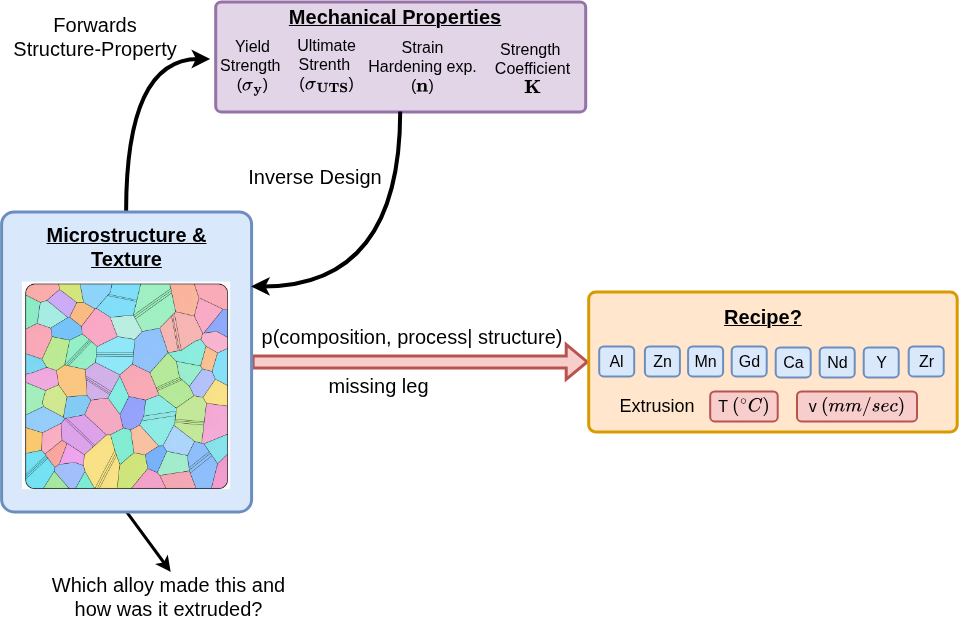
\includegraphics[width=0.99\linewidth]{figures/fig1_missing_leg.png}
  \caption{Microstructure and texture sit at the centre of alloy development:
  forward structure-to-property prediction and property-targeted inverse
  design are established, but turning an optimized structure back into a
  recipe (red) still leans on expert knowledge. This paper studies that leg:
  which alloy composition, what process parameters?}
  \label{fig:missing_leg}
\end{figure}

This is not an academic puzzle. In automated characterization pipelines and
self-driving laboratories, recovering the recipe from an optimized
microstructure is quality control, anomaly detection, and feed-forward
information for the next experiment \cite{Tom2024,Lee2026,Adesiji,Kalinin2021,Kalinin2022DeepLF}. It is also
the realistic first question in reverse engineering of legacy or competitor
materials. What makes it hard in practice is exactly what the workshop theme
calls the messiness of real experiments: measured campaigns are small,
heterogeneous, pooled across sources, and thinly sampled along every axis a
model would want to learn. We embrace that regime rather than simulate our way out of it. We demonstrate
on a measured dataset from our own previous work on wrought magnesium alloys, an
HCP system processed by extrusion: 107 extrusion conditions over 14 alloy
classes, with optical micrographs and X-ray diffraction texture per condition \cite{Guru2025}. Along the composition axis the
labels live on a discrete lattice of 14 alloys over an 8-element simplex; along
the process axis they live on a small catalogue of observed (temperature,
velocity) pairs. Both label spaces are discrete, and this single observation
drives everything that follows.

Three representation families are benchmarked for metallic microstructure, from
handcrafted statistics to a frozen vision embedding from a generative
foundation model to a learned grain-graph embedding, and pair them with
prediction heads that either respect or ignore the discrete label structure.
The question we put to each branch is not accuracy in the abstract but
\emph{compatibility}: does this way of describing an optimized microstructure
and texture support recovering the recipe behind it? The headline findings:

\begin{enumerate}[leftmargin=1.4em,itemsep=1pt]
  \item \textbf{Head structure beats representation scale.} On composition,
  handcrafted descriptors with a lattice-aware reranker reach 13.6\%
  present-element WAPE and 0.65 alloy top-1; the 1280-D vision and 128-D graph embedding
  embedding is three times worse.
  \item \textbf{The process window is a catalogue, not a continuum.} Decoding
  a correlated Gaussian process over the grid of observed training conditions,
  in both temperature and speed, beats continuous regression on velocity for
  every representation we report.
  \item \textbf{Selection must be honest to be believed.} The winning head is
  chosen by out-of-fold constraints on all-element WAPE and false-positive
  rate.
  \item \textbf{Compatibility is measurable.} We offer
  compatibility of descriptor to prediction head, as the right criterion for
  choosing representations in small experimental campaigns.
\end{enumerate}

\section{Data: sparse by construction}
\label{sec:data}

The dataset aggregates measured extrusion campaigns
of wrought magnesium alloys: AZ31 from a doctoral thesis
\cite{nienaber_einfluss_der_2023} and a processing-parameter study
\cite{Nienaber2019}, the Zn-bearing alloys Z1, ZX10 and ZNd10 from a Zn-bearing
extrusion study \cite{CANOCASTILLO2020139527,Nienaber2019}, ME21 from an
extrusion-parameter study \cite{KurzG}, and the Mg-Gd family Mg-2/5/10Gd with
0, 0.5, or 1 wt\% Mn micro-additions from Mg-Gd and Mg-Gd-Mn extrusion studies
\cite{Harmuth,cryst12081036}. Each of the 107 conditions combines a base alloy (composition
in wt\% over the 8-element lattice Al, Zn, Mn, Ce, Gd, Ca, Nd, Y), an extrusion
temperature $\Text \in [200, 500]$\,°C, and a ram speed $\vext \in [0.5,
7.5]$\,mm/s. Per condition we have optical micrographs (15 to 108 images after
segmentation quality control) and X-ray pole figures reduced to an orientation
distribution function (ODF).

\paragraph{Two kinds of sparsity.} The composition axis is sparse because 14
alloys barely populate an 8-element simplex; most elements are zero in most
alloys, and Y appears in exactly one. The process axis is sparse and
\emph{confounded}: each alloy family was extruded on its own temperature-speed
sub-grid, so process and composition are correlated by experimental design.
Any model can exploit that correlation; the honest question is whether it can
also move \emph{within} a family.

\paragraph{Two symmetric tasks.} We decompose structure-to-recipe into two
conditionally complete tasks. \textbf{Task A (composition):} given the
structure representation plus the known process $(\Text, \log \vext)$ and an
extrusion-ratio-type flag, predict the element wt\% vector.
\textbf{Task B (process):} given the representation plus the known composition
and the same flag, predict $(\Text, \vext)$. Each task sees exactly the half of
the recipe a deployment would already know, mirroring how an alloy's family is
known once an optimized microstructure exists.

Repeated images of one condition make random
image-level splits meaningless: the same condition's CatBoost+kNN fusion scores
100\% alloy top-1 under such a split. All results here therefore use
condition-grouped 5-fold cross-validation: every condition (all its images)
sits in exactly one held-out fold, folds are formed over the 107 conditions,
and test folds are touched once. Validation portions select base
hyperparameters only; all winner selection happens on training out-of-fold
predictions (Section~\ref{sec:heads}).

\section{Three ways to describe a microstructure}
\label{sec:repr}

Figure~\ref{fig:pipeline} shows the three descriptor branches. They span the
design space a practitioner actually faces, from classical statistics to
vision embeddings, and the benchmark asks which of them is
\emph{compatible} with recipe inference at 107 conditions.

\begin{figure}[t]
  \centering
  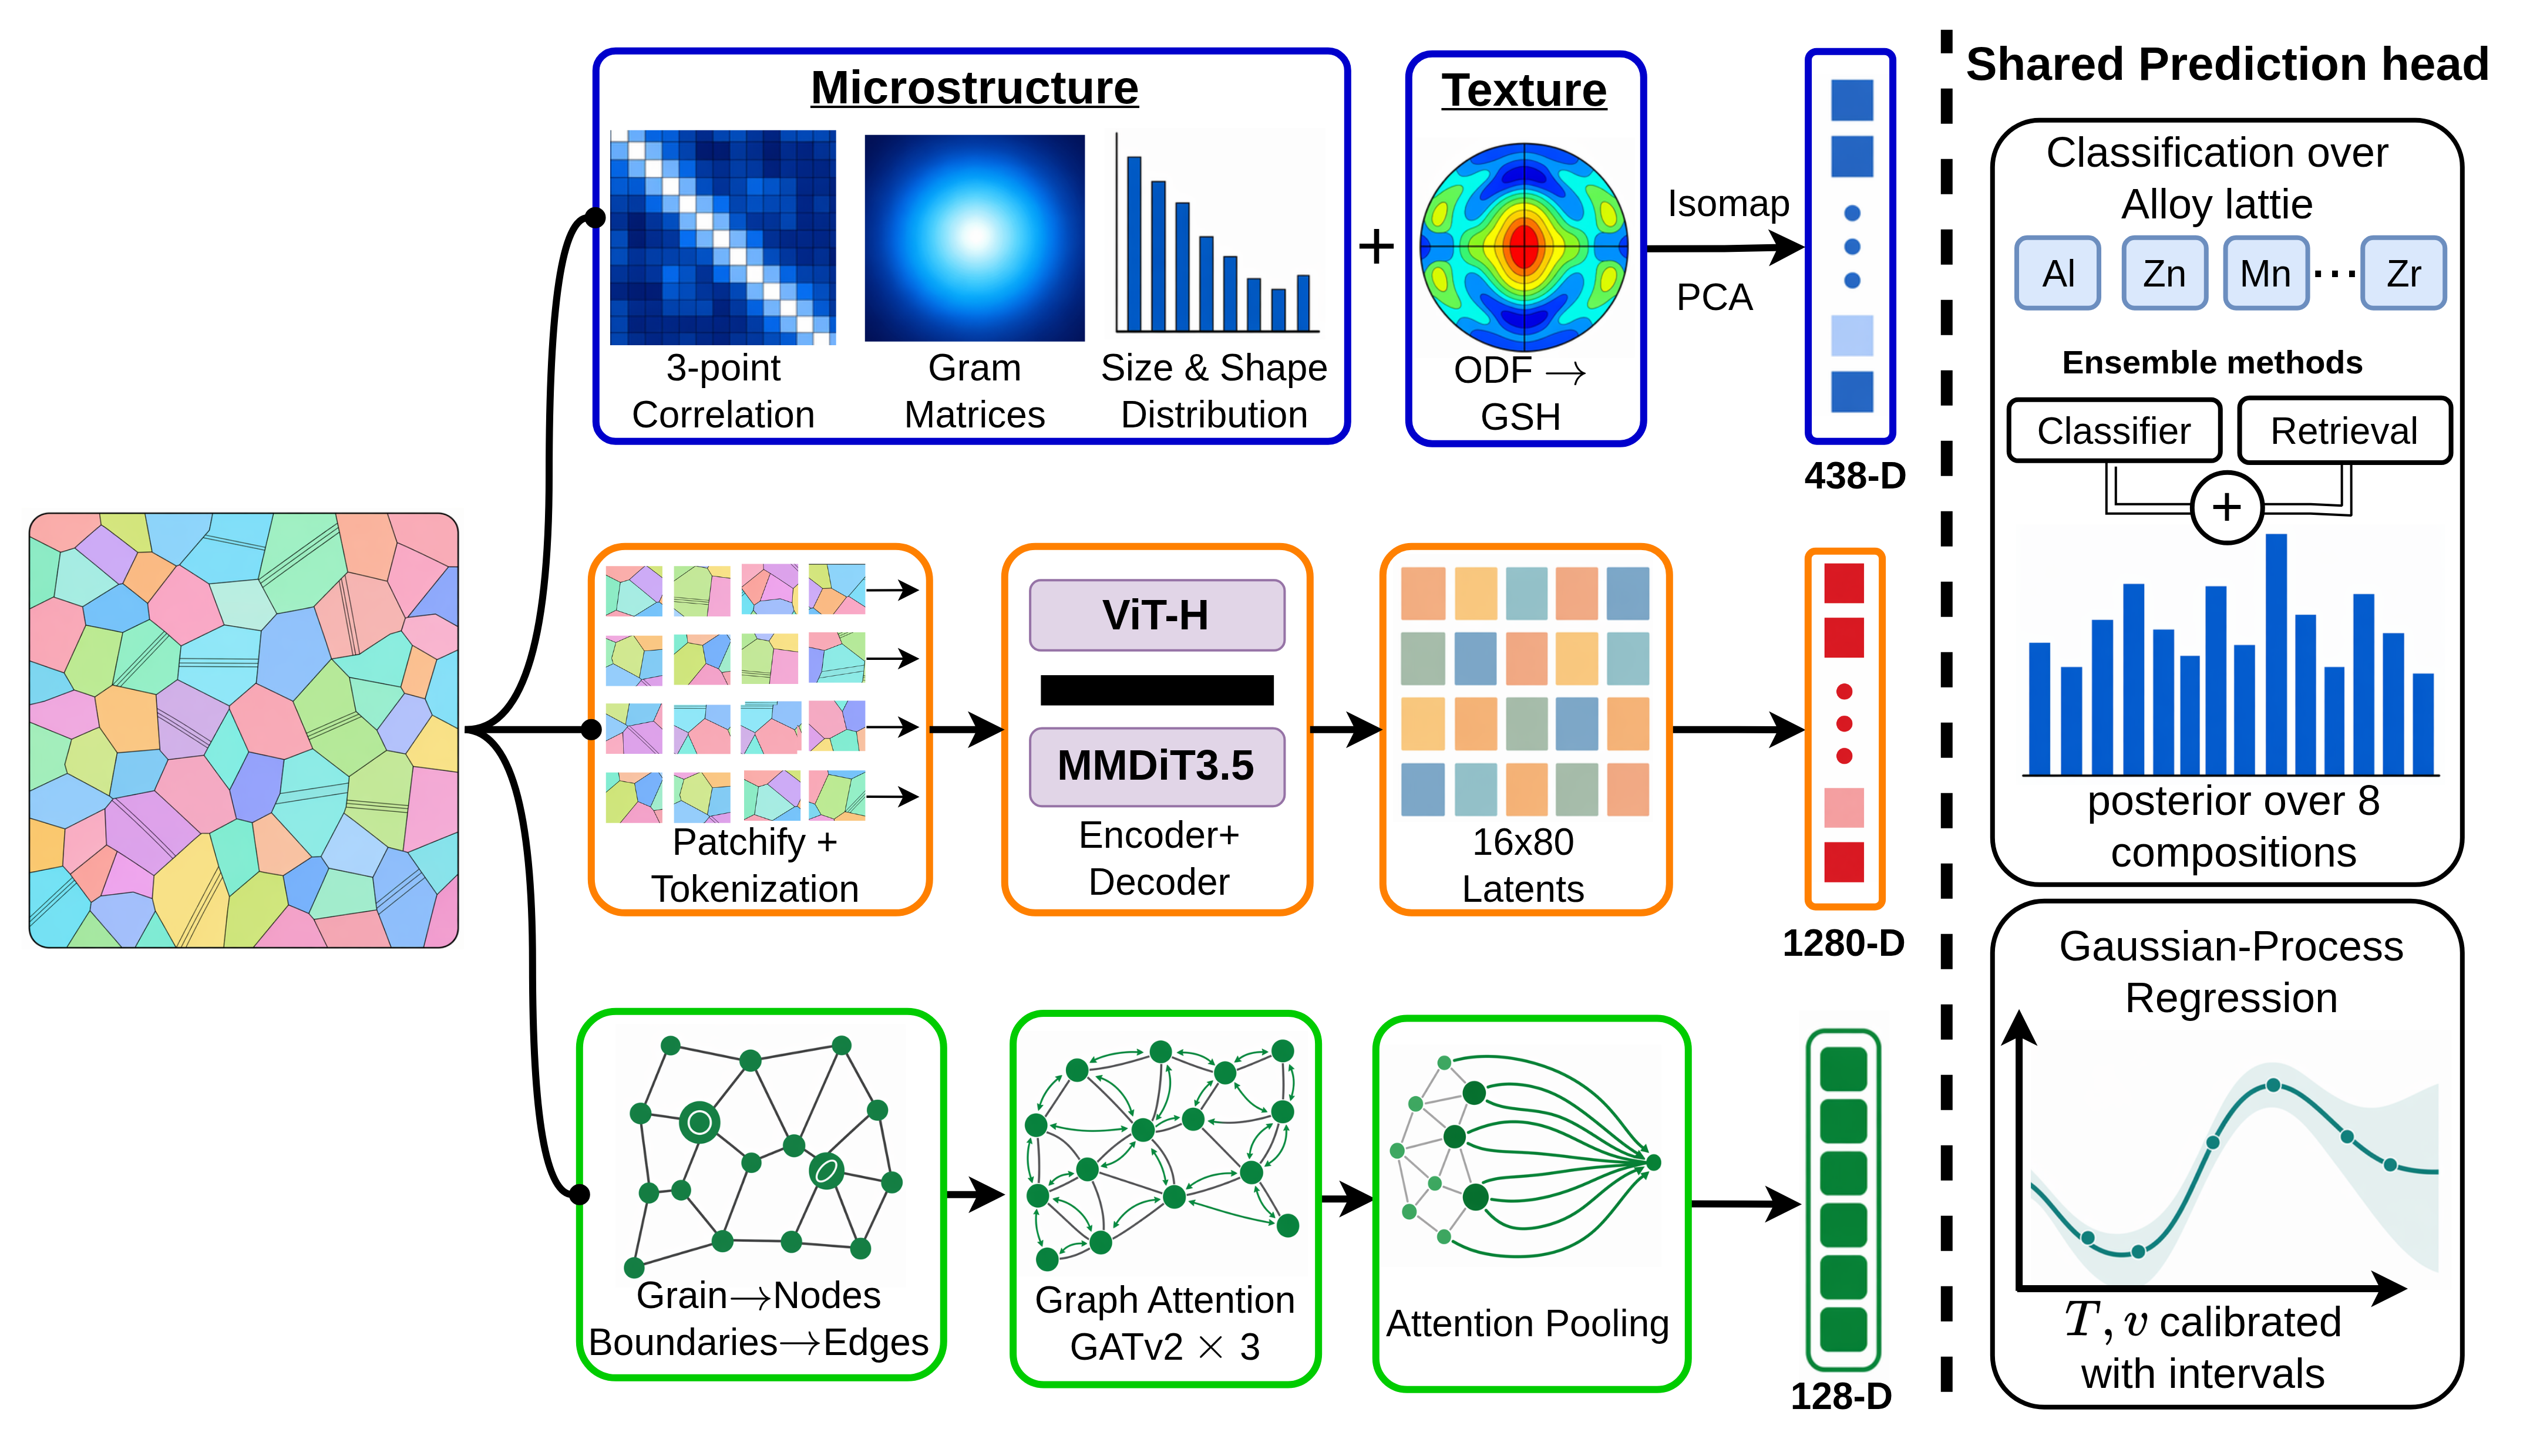
\includegraphics[width=\linewidth]{figures/fig2_pipeline.png}
  \caption{Three descriptor branches with shared prediction heads.
  \textbf{Top (blue):} handcrafted microstructure and texture statistics,
  438-D. \textbf{Middle (orange):} frozen ViT-H encoder with an MMDiT
  diffusion decoder, 1280-D
  (Figure~\ref{fig:vision}). \textbf{Bottom (green):} grain adjacency graph
  through a GATv2 encoder with attention pooling, 128-D. Right: the shared
  heads.}
  \label{fig:pipeline}
\end{figure}

\paragraph{Conventional statistics (438-D).} Following the forward-modeling
pipeline of \cite{Guru2025}, each image contributes:
PCA-reduced 3-point spatial correlations (120-D), Isomap-reduced Gram matrices
of pretrained CNN activations (200-D), aspect-ratio and equivalent-diameter
distributions (58-D), and from the ODF, Isomap-reduced generalized spherical
harmonics coefficients (60-D). These descriptors are cheap, deterministic, and
were designed by domain knowledge about what distinguishes one extruded
microstructure from another \cite{Kalidindi-MKS-2015,markley2007,tenenbaum2000isomap,gatys2015texture,gatys2016style}.

\paragraph{Vision embedding (1280-D).} The middle branch reuses the frozen
encoder-decoder of our companion work which is under review, trained on $\sim$80k EBSD-derived microstructures. A
ViT-H/14 trunk \cite{dosovitskiy2021image} initialized from
natural-image CLIP weights \cite{radford2021clip}, its lower
half frozen and its upper 16 blocks fine-tuned, is read out by a multi-query
attention pooler into 16 spatial latent tokens, and a frozen Stable
Diffusion 3.5 MMDiT decoder arm \cite{esser2024sd3}
is trained jointly with the encoder to reconstruct the micrograph, so the
latent is shaped by a composite of generative and alignment terms
\cite{peebles2023dit,lipman2023flowmatching}. The
$16 \times 80$ latent tokens are flattened to the 1280-D vision embedding
(Figure~\ref{fig:vision}). We deliberately do not retrain anything here: the
question is whether a vision embedding shaped for \emph{generation and
reconstruction} transfers to \emph{recipe inference}. Architecture and training
detail are in the companion paper; what matters here is only that this is the
strongest generative representation of these microstructures available to us.

\begin{figure}[t]
  \centering
  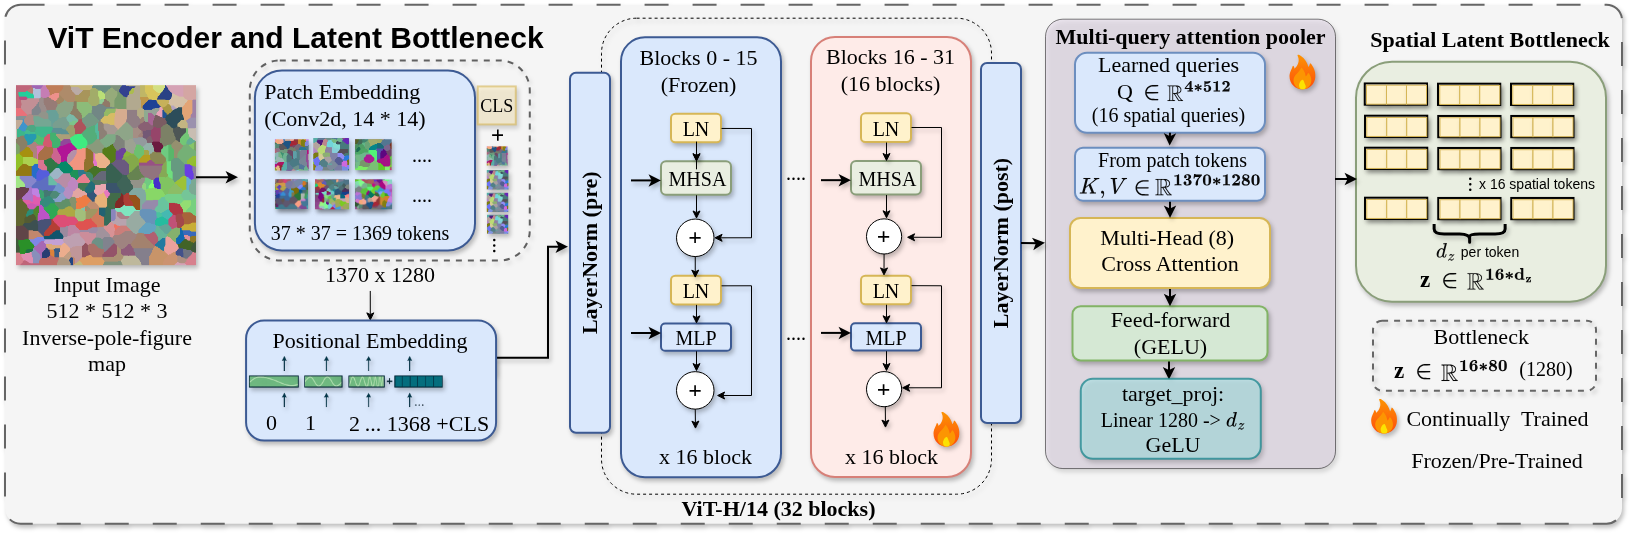
\includegraphics[width=0.99\linewidth]{figures/fig_vision_embedding.png}
  \caption{The vision-embedding branch. A micrograph is patchified and encoded
  by the ViT-H encoder into the latent the MMDiT decoder reconstructs from;
  the $16 \times 80$ latents serve, frozen, as the 1280-D representation.}
  \label{fig:vision}
\end{figure}

\paragraph{Grain-graph embedding (128-D).}
\label{sec:gnn}
The third branch builds a grain
adjacency graph per image and encodes it with a graph attention network.
Figure~\ref{fig:gnn} shows the four stages. Each segmented micrograph becomes
a graph whose nodes are grains and whose edges are shared boundaries \cite{groeber2014}.
Node features cover grain geometry and orientation (area, aspect ratio,
Bunge-Euler angles, centroid, bounding box); edge features are shared-boundary
length and misorientation angle \cite{randle2001grain}. A linear projection to 128-D is followed by four GATv2 attention
blocks (4 heads, edge dimension 2, LayerNorm + GELU + residual) \cite{brody2022how, velickovic2018graph, vaswani2017attention}, and attention pooling with 8 learned
seed queries produces 8 microstructure tokens of 128-D per image, mean-pooled
to the 128-D embedding used in the benchmark. The encoder is trained with the
flow-matching objective of the companion pipeline and then frozen; per fold we
reuse the cached embeddings.

\begin{figure}[t]
  \centering
  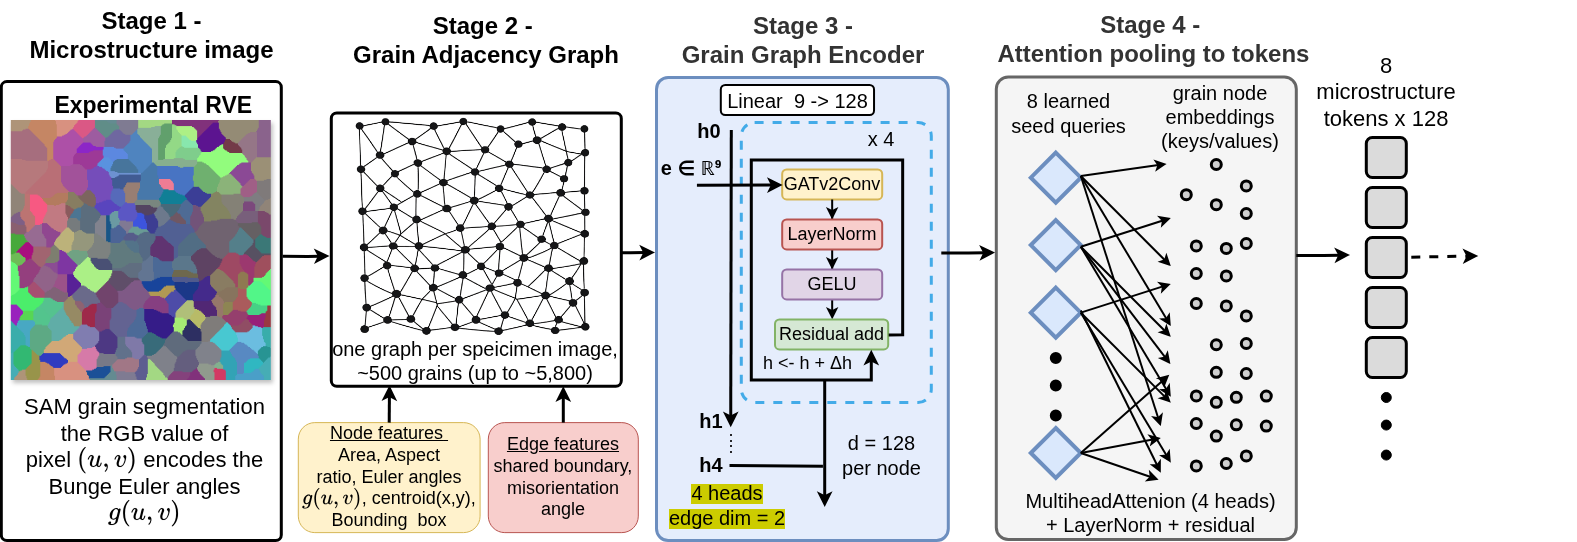
\includegraphics[width=\linewidth]{figures/fig3_gnn.png}
  \caption{Grain-graph encoder. Stage 1: segmented microstructure. Stage 2:
  grain adjacency graph, roughly 500 grains per image. Stage 3: four GATv2
  blocks with residual connections. Stage 4: attention pooling to 8
  microstructure tokens.}
  \label{fig:gnn}
\end{figure}

\section{Heads that match the label space}
\label{sec:heads}

Both label spaces are small and discrete. The composition label is one of 14
nominal alloy vectors; the process label is one of the observed $(\Text,
\log \vext)$ pairs in the training folds. We therefore compare, per task, heads
that exploit this structure against strong continuous baselines.

\paragraph{Task A: composition as lattice classification.} Three heads.
(i) \textbf{kNN retrieval}: soft voting over the nearest training images in
the representation, the natural retrieval baseline on a small lattice \cite{cover1967nearest, wang2014learning}.
(ii) \textbf{Condition-balanced fusion}: a 14-way CatBoost classifier and the
kNN vote, each with equal total training weight per condition, blended 50:50 \cite{prokhorenkova2018catboost,friedman2001greedy, chen2016xgboost}.
(iii) \textbf{OOF-constrained reranker}: the fusion is the \emph{owner}; on the
conventional branch, five per-descriptor-block logistic classifiers on
condition-mean features act as a complementary \emph{auxiliary}
\cite{hastie2009elements}, and the final
posterior is a convex blend
$p = w\, p_{\mathrm{owner}} + (1-w)\, p_{\mathrm{aux}}$.
The weight $w$ is selected on training out-of-fold predictions only, and a
candidate $w$ is eligible only if it does not degrade all-element WAPE or the
false-positive rate relative to the owner \cite{wolpert1992stacked, varma2006bias}. On
the vision and gnn branches, which
have no descriptor blocks, an FT-Transformer classifier plays the auxiliary
role \cite{gorishniy2021revisiting, badaro2023transformers}.

\paragraph{Guard metrics.} The deployment question behind Task A is the
\emph{levels} of the elements in a known alloy family, so the headline metric
is present-element WAPE (weighted absolute percentage error over elements
actually present, reported throughout simply as WAPE). WAPE alone is gameable:
a head that predicts every element as present scores deceptively well. Every
composition row therefore also reports all-element WAPE and the macro
false-positive rate. This guard discipline is not cosmetic: in our own
head-search history, several metric-learning and hurdle heads posted attractive
WAPE values while predicting 12-37\% false-positive elements
(Section~\ref{sec:results}).

\paragraph{Task B: process as catalogue decoding.} Three heads.
(i) \textbf{GBDT}: gradient-boosted decision trees (CatBoost, targets
standardized, $\vext$ in log space). (ii) \textbf{Gaussian process}:
condition-pooled features, PCA-32, anisotropic RBF kernel, lognormal treatment
of $\vext$ with the smearing correction \cite{rasmussen2006gaussian, duan1983smearing}.
(iii) \textbf{Joint-grid GP}: a correlated GP over the joint latent
$(\Text, \log \vext)$, whose posterior at a query is decoded by minimum-risk
selection over the discrete grid of observed training pairs rather than read
off continuously \cite{eikema2022sampling}.
The same catalogue constraint is applied to velocity: extrusion speed is set
from a short menu of press settings, so a value between two settings is never a
possible answer, and the continuous estimate is snapped onto the observed
levels, nearest in log space. Which continuous estimate feeds that snap is
chosen on training out-of-fold predictions, optionally blended with an ordinal
classifier over velocity levels or the grid posterior median, under safety
constraints that forbid degrading the plain snapped log-GP fallback.

\section{Results}
\label{sec:results}

\paragraph{Task A: composition.} Table~\ref{tab:composition} collects the
5-fold results. The conventional reranker wins outright: 13.6\% WAPE against
16.8\% for its own owner and 30.0\% for retrieval, with the best top-1 (0.646)
the fewest false positives (1.1\%), and the sharpest posterior (class NLL
1.38). The
descriptor-block auxiliary genuinely complements the owner on this branch. On
the learned representations the same machinery honestly reports failure: the
out-of-fold selection chooses owner weight 1.0 on 8 of 10 vision/gnn folds,
i.e. the auxiliary adds nothing and the head correctly refuses to use it.
Figure~\ref{fig:confidence} shows what sits underneath: the conventional head
is confidently right on a large share of conditions, while both learned
embeddings assign almost no probability to the truth on much of the lattice,
the mechanism behind their NLL near 2.3.

\begin{figure}[t]
  \centering
  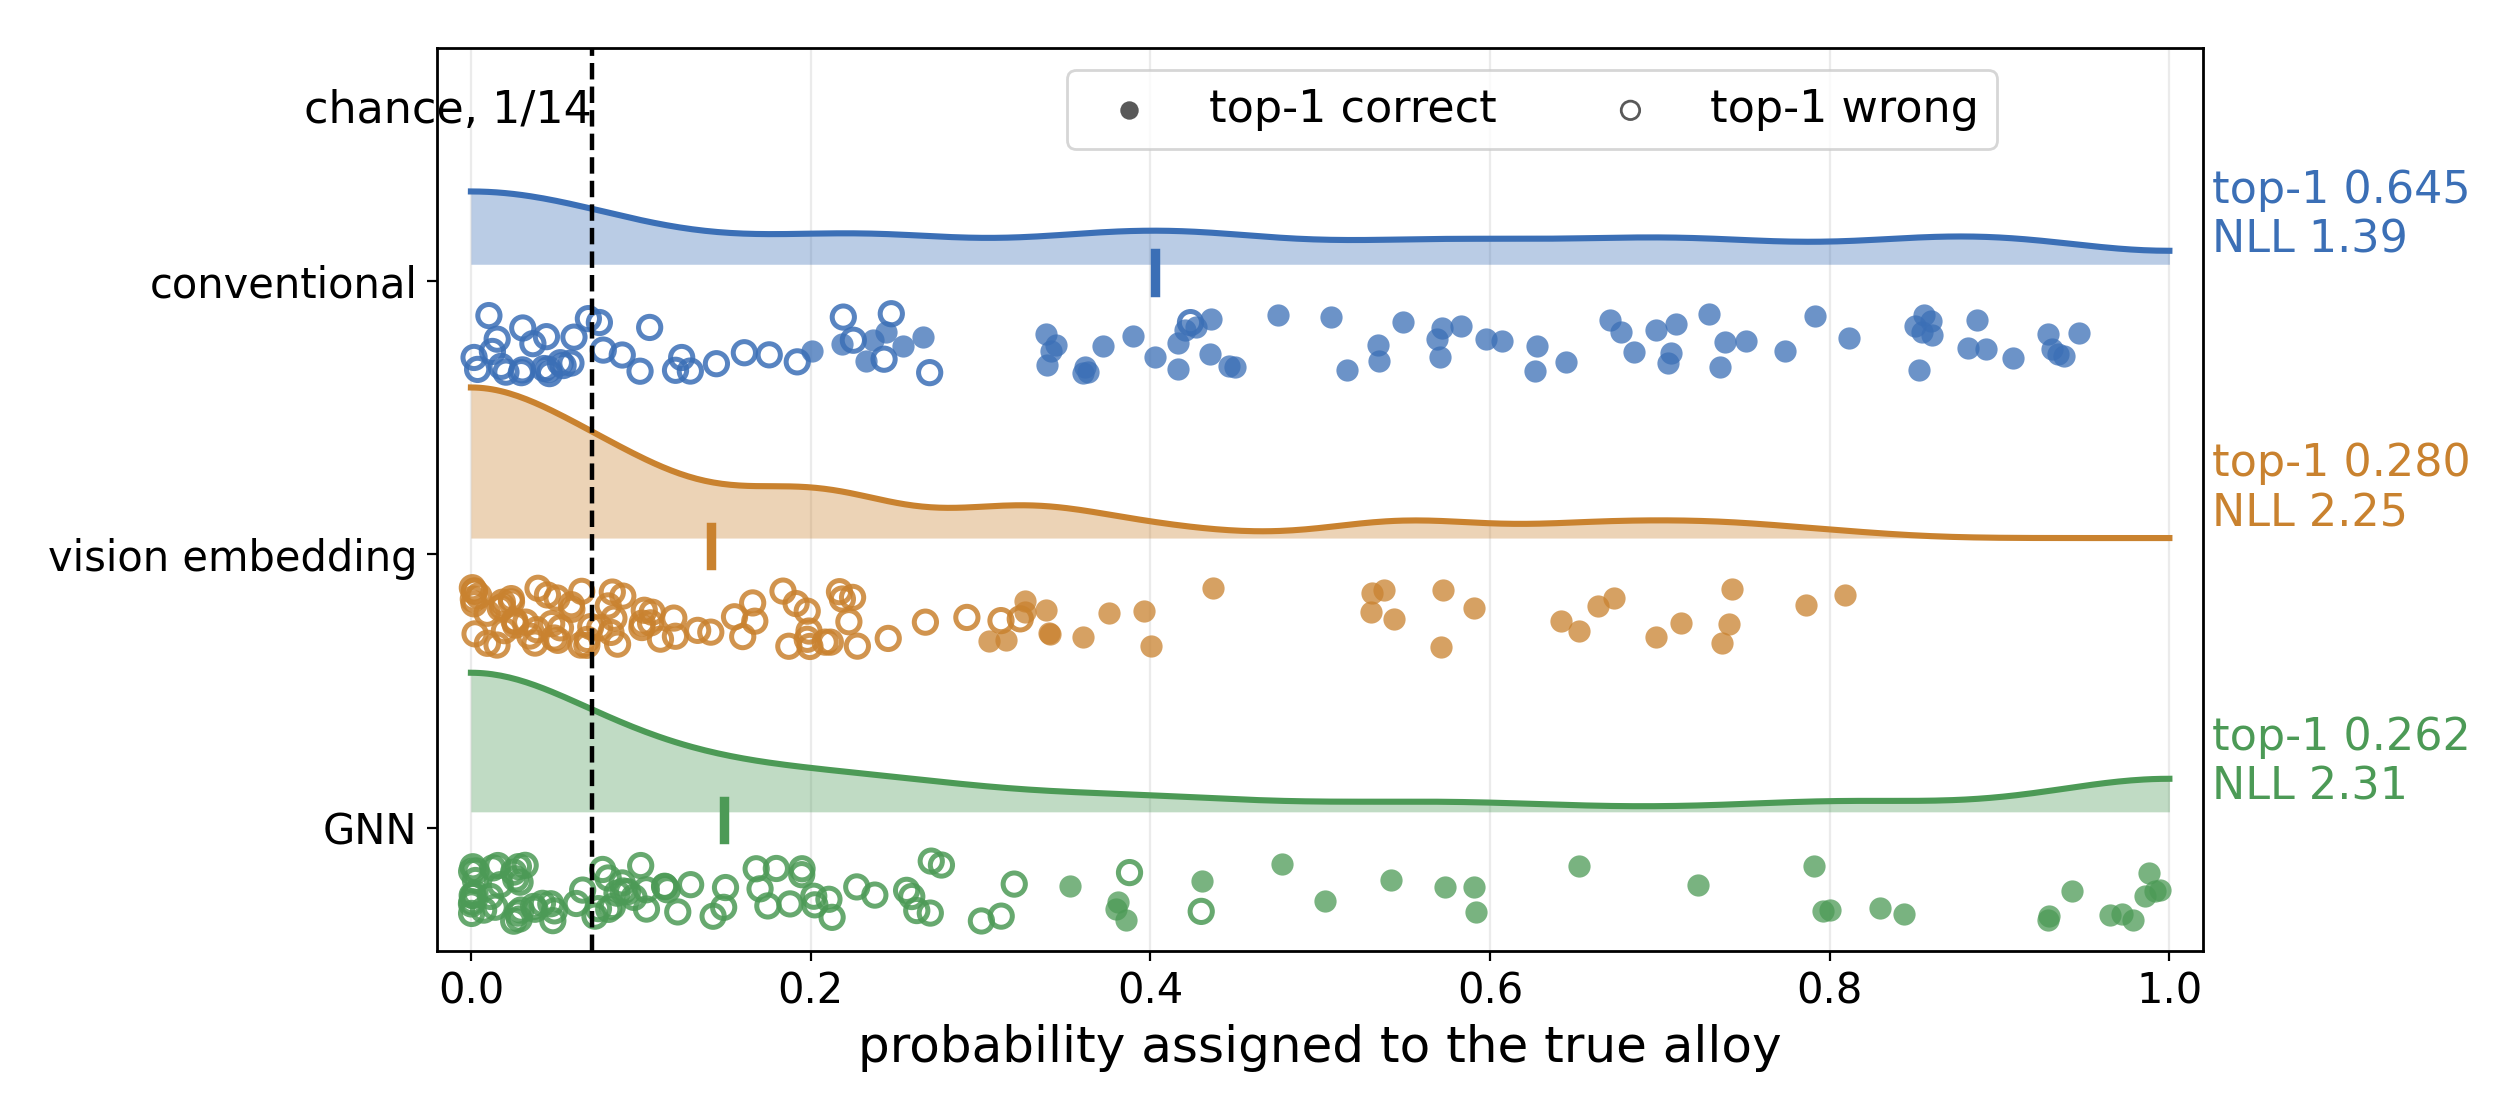
\includegraphics[width=0.99\linewidth]{figures/fig_composition_confidence.png}
  \caption{Task A confidence: the probability the reranker assigns to the true
  alloy, pooled over all 107 held-out conditions. Density above each line, one
  dot per condition below (filled = top-1 correct, open = wrong), tick =
  median, dashed = chance ($1/14$). Annotations match Table~\ref{tab:composition}.}
  \label{fig:confidence}
\end{figure}

\begin{table}[t]
  \caption{Task A, composition given known process. 5-fold cross-validation,
  mean $\pm$ std over held-out condition groups. WAPE = present-element WAPE;
  FP = false-positive rate; top-1 = alloy accuracy; NLL = class
  log-likelihood. Best per column in bold.}
  \label{tab:composition}
  \centering\small
  \begin{tabularx}{\linewidth}{@{}llXXXX@{}}
    \toprule
    repr. & head & WAPE (\%) & FP (\%) & top-1 & NLL \\
    \midrule
    \multirow{3}{*}{conv.}
      & kNN retrieval & $30.0 \pm 7.6$ & 10.3 & $0.496 \pm 0.110$ & 5.92 \\
      & balanced fusion & $16.8 \pm 5.8$ & 1.3 & $0.612 \pm 0.078$ & 1.49 \\
      & OOF-constrained reranker & $\mathbf{13.6 \pm 4.1}$ & \textbf{1.1} & $\mathbf{0.646 \pm 0.051}$ & \textbf{1.38} \\
    \midrule
    \multirow{2}{*}{vision}
      & balanced fusion & $44.7 \pm 18.0$ & 6.5 & $0.276 \pm 0.104$ & 2.25 \\
      & OOF-constrained reranker & $41.6 \pm 18.9$ & 5.9 & $0.287 \pm 0.111$ & 2.23 \\
    \midrule
    \multirow{2}{*}{gnn}
      & balanced fusion & $44.3 \pm 8.0$ & 7.2 & $0.266 \pm 0.071$ & 2.34 \\
      & OOF-constrained reranker & $44.2 \pm 8.0$ & 7.2 & $0.266 \pm 0.071$ & 2.30 \\
    \bottomrule
  \end{tabularx}
\end{table}

\paragraph{Task B: process.} Table~\ref{tab:process} shows the mirror task.
Because velocity lives on a discrete menu, the headline number is how often the
right setting is recovered: the joint-grid GP names the exact press speed on
24-29\% of held-out conditions and lands within one setting on 46-52\%, against
a 9\% chance level, and it also wins every regression metric (MAPE
48.7, 49.6, 51.4\% against a 136.5\% constant-predictor floor). It also gives
the best temperature on conventional and vision. The plain continuous GP
collapses on velocity (MAPE 95-120\%): the improvement comes from decoding on
the observed grid, not from the GP itself.
This is the process-side analogue of the composition lattice: with roughly 70
training conditions per fold, the process label is better treated as a small
catalogue than as a continuum. Figure~\ref{fig:temp_parity} shows the
predicted-versus-true view for temperature: both heads track the diagonal but
saturate above $\approx 400$\degC, and the joint-grid GP's latent intervals
cover the diagonal on most held-out conditions.

\begin{figure}[t]
  \centering
  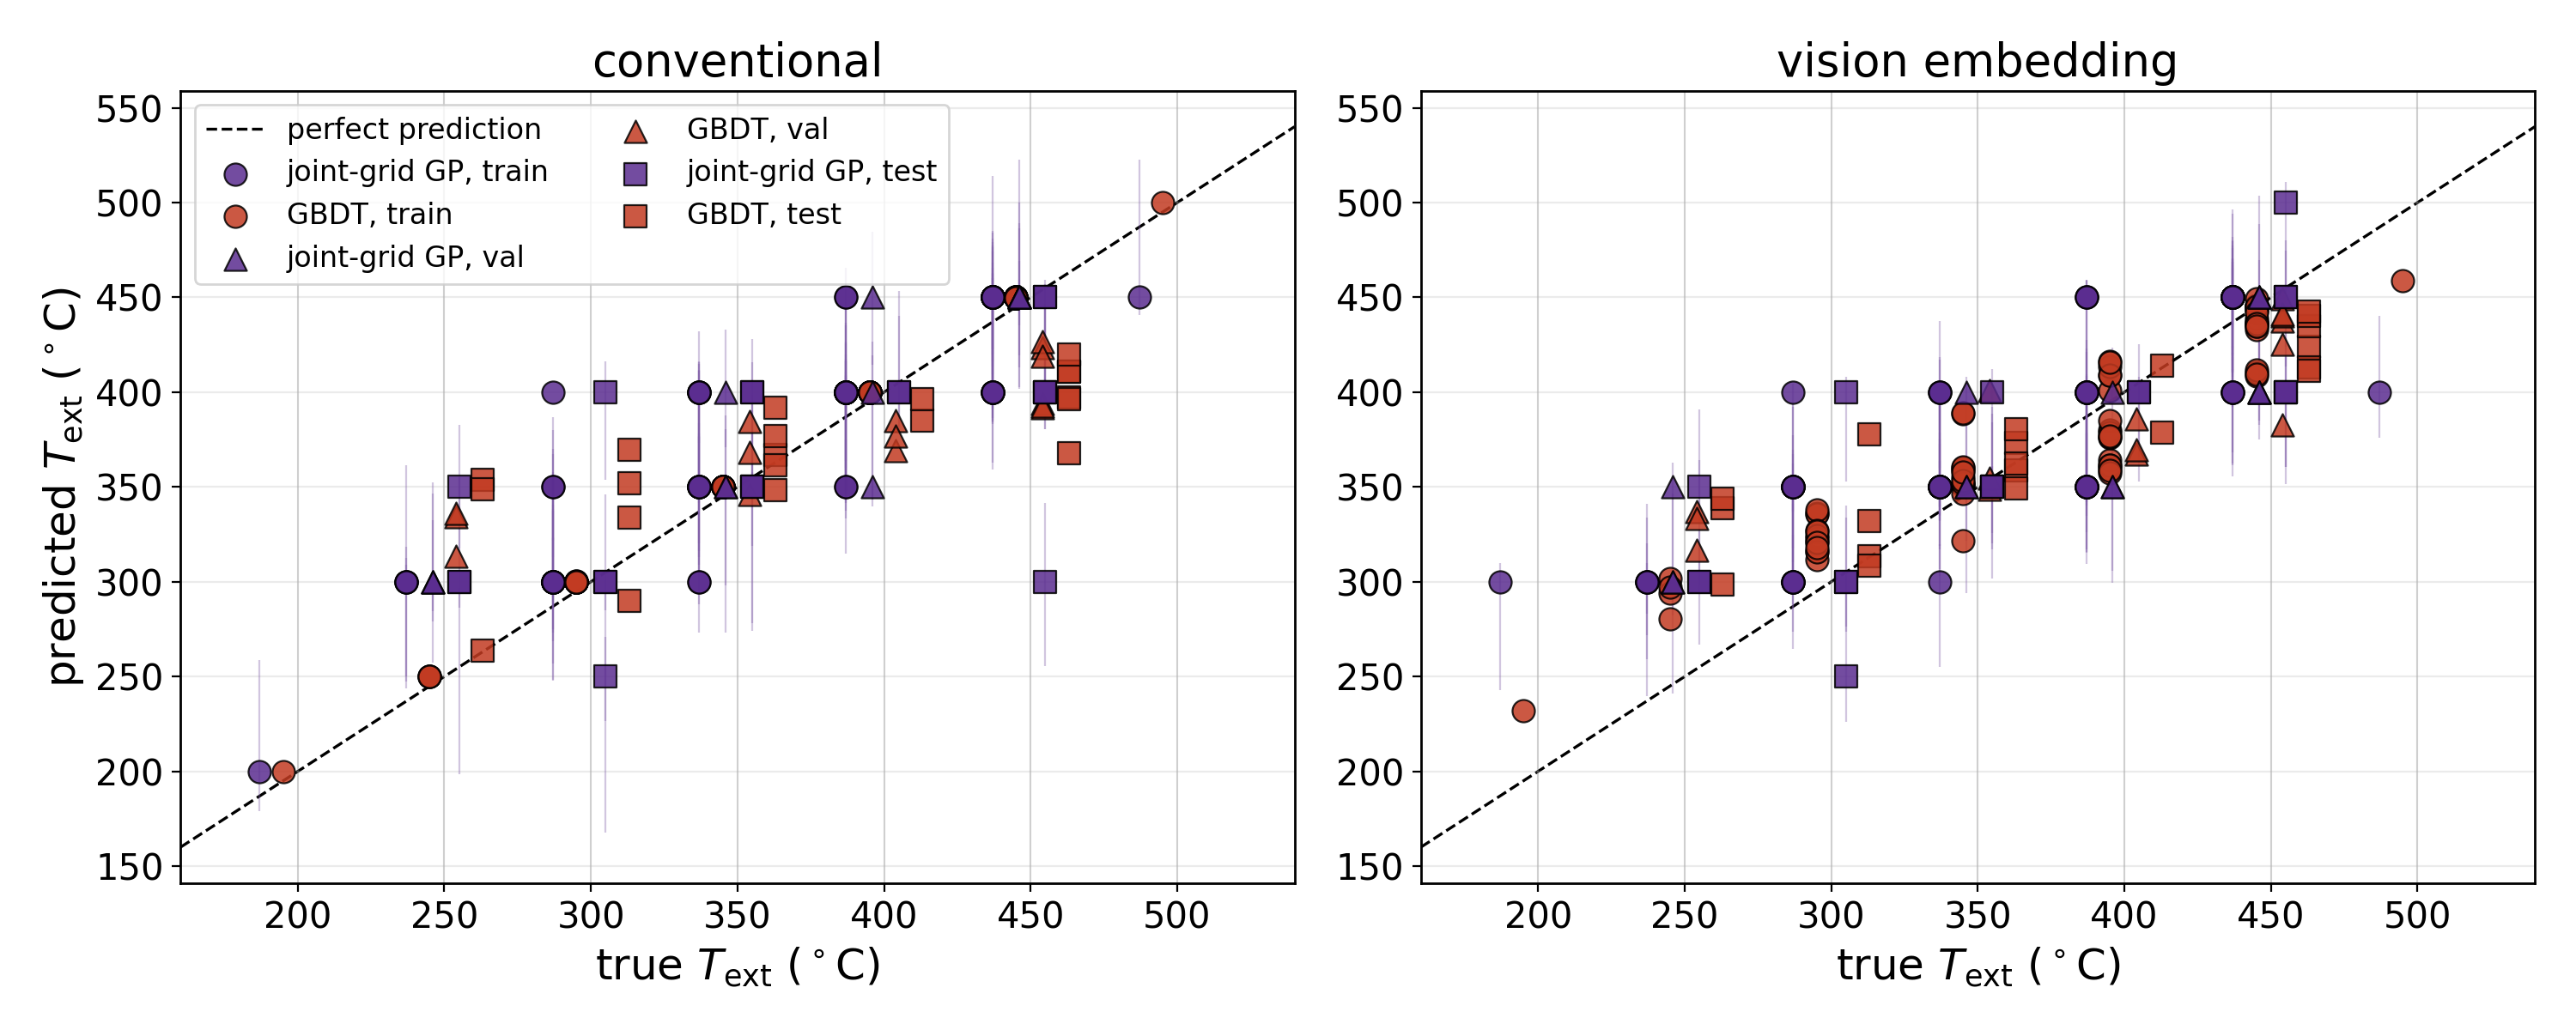
\includegraphics[width=0.99\linewidth]{figures/fig_temperature_parity.png}
  \caption{Task B temperature: predicted against true $\Text$
  (\texttt{cv\_fold0}). Purple = joint-grid GP (bar = latent 90\% interval),
  red = GBDT; circles / triangles / squares = train / val / test, dashed =
  perfect prediction. Both heads saturate at the high-temperature end.}
  \label{fig:temp_parity}
\end{figure}

\paragraph{Velocity is a log-scale quantity.} Extrusion speed spans 0.5 to
7.5\,mm/s over eleven distinct settings, so raw MAE flatters a head that simply
predicts near the middle of the range and MAPE punishes it only at the slow end.
We therefore also report error in log space, where a fixed error means a fixed
multiplicative factor everywhere on the range. The picture is consistent with
the raw numbers but sharper: the joint-grid GP reaches a log MAE of 0.42-0.45
across the three representations, a typical multiplicative error of about
1.53-1.58$\times$, against 0.63-0.75 (1.88-2.17$\times$) for the continuous GP.
Only in log space is the continuous GP's failure fully visible: its log error is
larger than the spread of log speeds across the catalogue, so on two of three
representations it is worse than predicting the training mean speed.
Figure~\ref{fig:vel_parity} makes the same point directly: the joint-grid GP
and GBDT are tight at low speed and spread at high speed, and the spread is
asymmetric, since the heads rarely overshoot a slow condition but often
undershoot a fast one.

\begin{figure}[t]
  \centering
  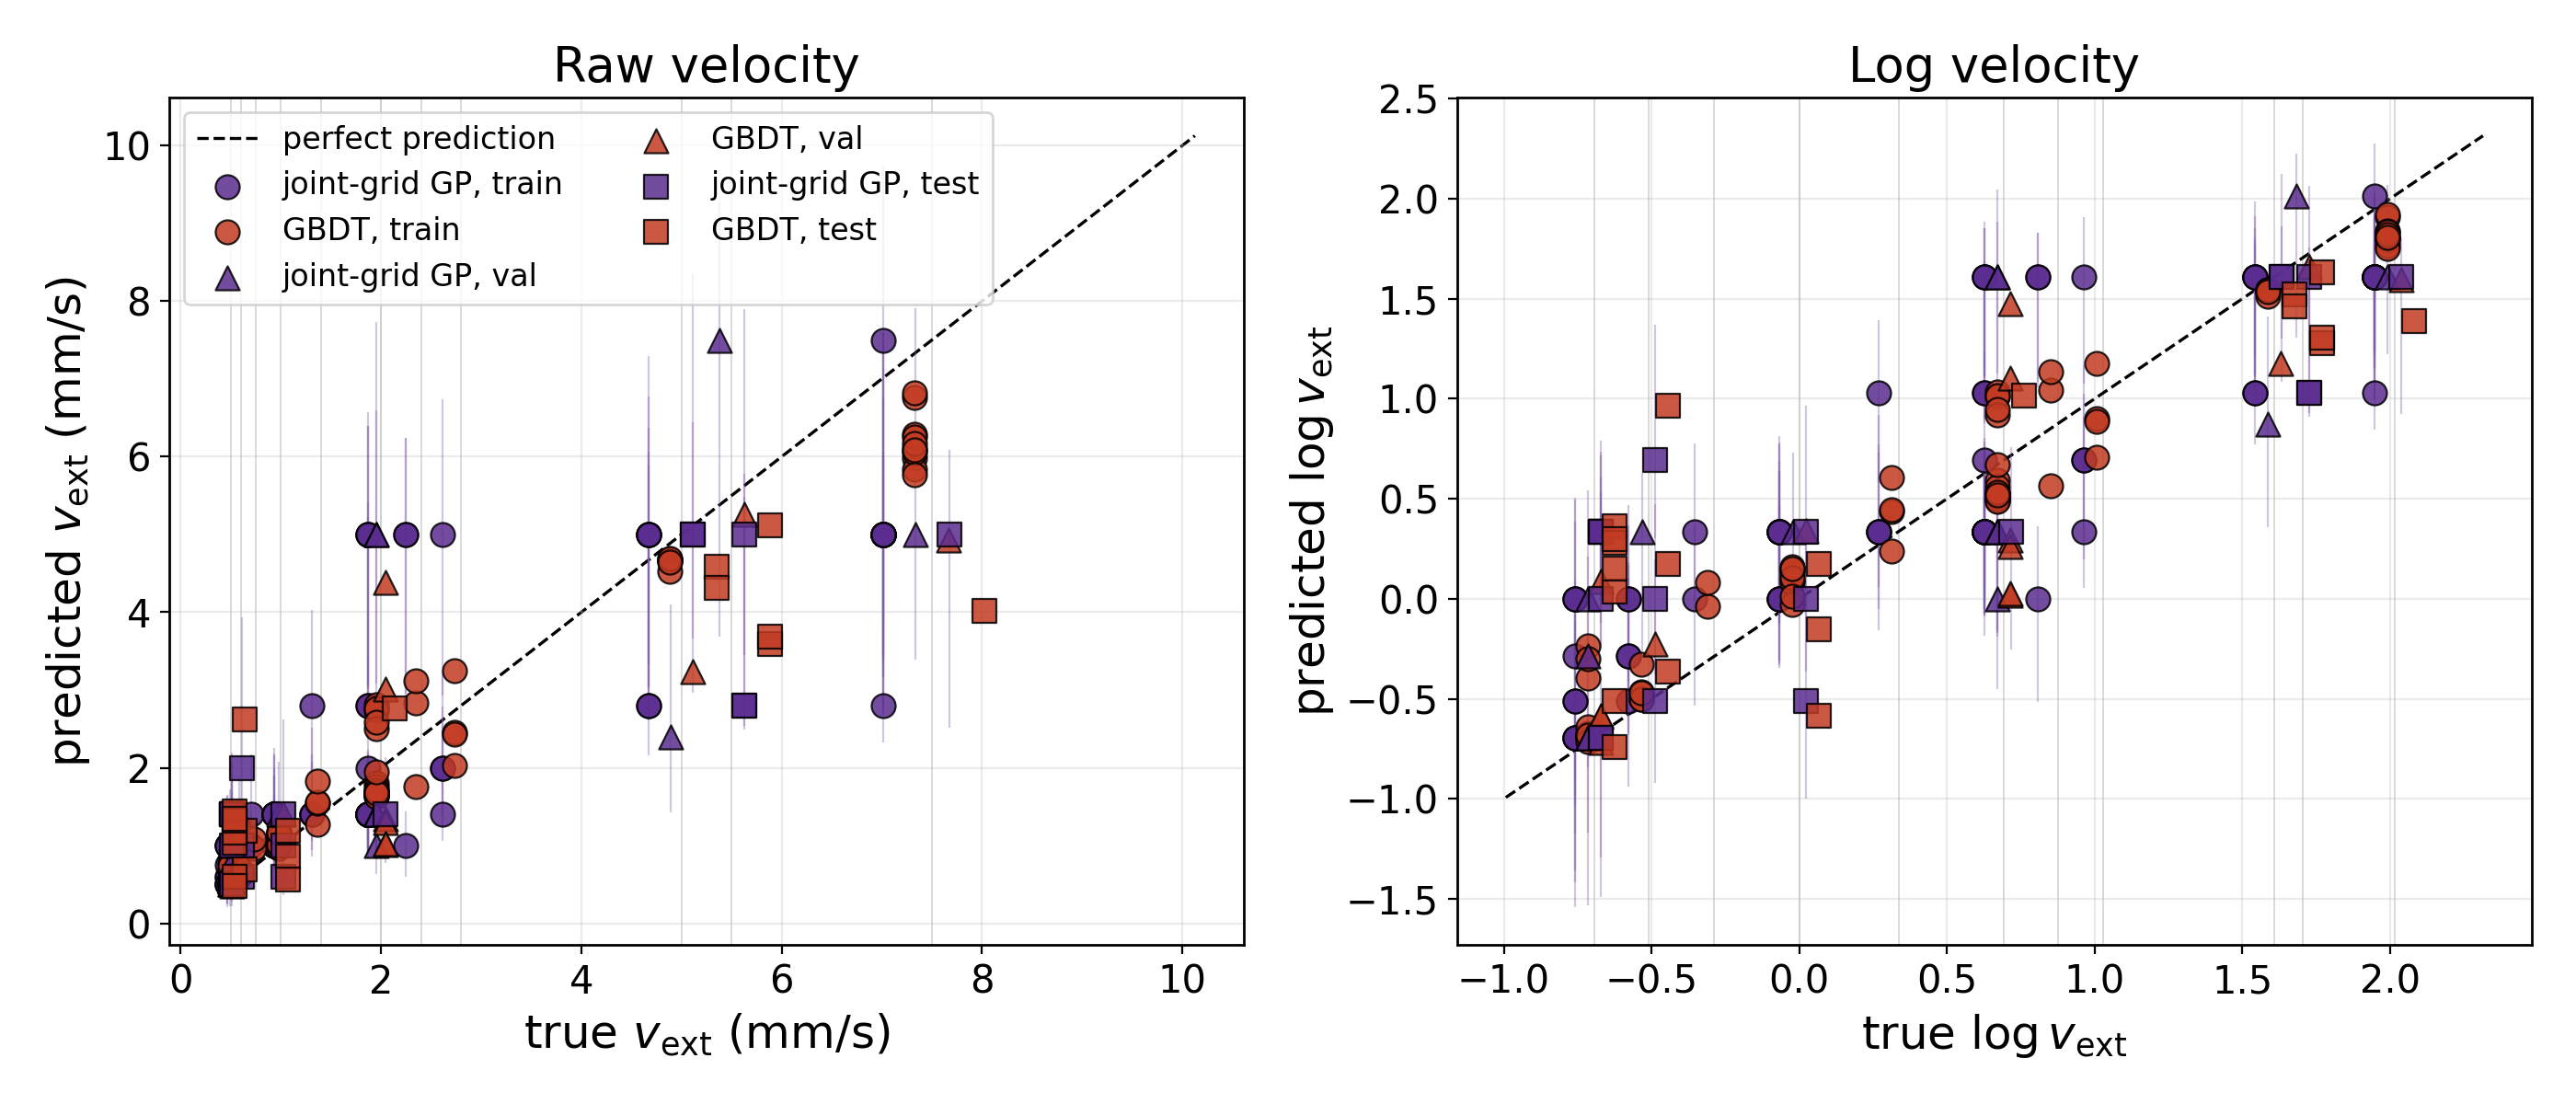
\includegraphics[width=0.99\linewidth]{figures/fig_gnn_velocity_parity.png}
  \caption{Task B velocity on the GNN branch (\texttt{cv\_fold0}), predicted
  against true $\vext$, raw (left) and log (right). Purple = joint-grid GP,
  red = GBDT, grey = observed press settings, dashed = perfect prediction.}
  \label{fig:vel_parity}
\end{figure}

\paragraph{The residual error is tail shrinkage, and it is not a capacity
problem.} Even the best head does not extrapolate to the edges of the catalogue.
On the conventional branch, the 26 fastest conditions (true $\vext \ge
5$\,mm/s, mean 6.3) are predicted at a mean of 4.4\,mm/s, and the 46 slowest
($\le 1$\,mm/s, mean 0.7) at 1.0\,mm/s: the model commits to the middle of the
observed menu and declines the extremes. This is a property of the label, not of
model depth. The heads already model $\vext$ in log space, snap to the
catalogue, and blend an ordinal tail classifier, yet none recovers the extreme
speeds, and a deliberately over-deep CatBoost does not beat them on held-out
conditions. With about two fast examples per alloy family, no regression depth
extracts a signal the features do not carry. This is the generic failure mode of
sparse experimental data: when a target is sampled at a few well-separated
settings, the honest estimate concentrates on the dense interior and the sparse
tails are smoothed away, however strong the learner. The remedy is information,
more extreme-setting conditions or features sensitive to the speed-controlled
recrystallization signature, not a larger model.
Figures~\ref{fig:lda_temperature} and \ref{fig:gnn_velocity} trace this
directly along a 1-D supervised projection of the head input: temperature and
velocity are both monotonic in the projection, and the two heads' mean
responses flatten at both ends of the range while the held-out points follow
the same trend, so the contraction is in the representation, not the head.

\begin{figure}[t]
  \centering
  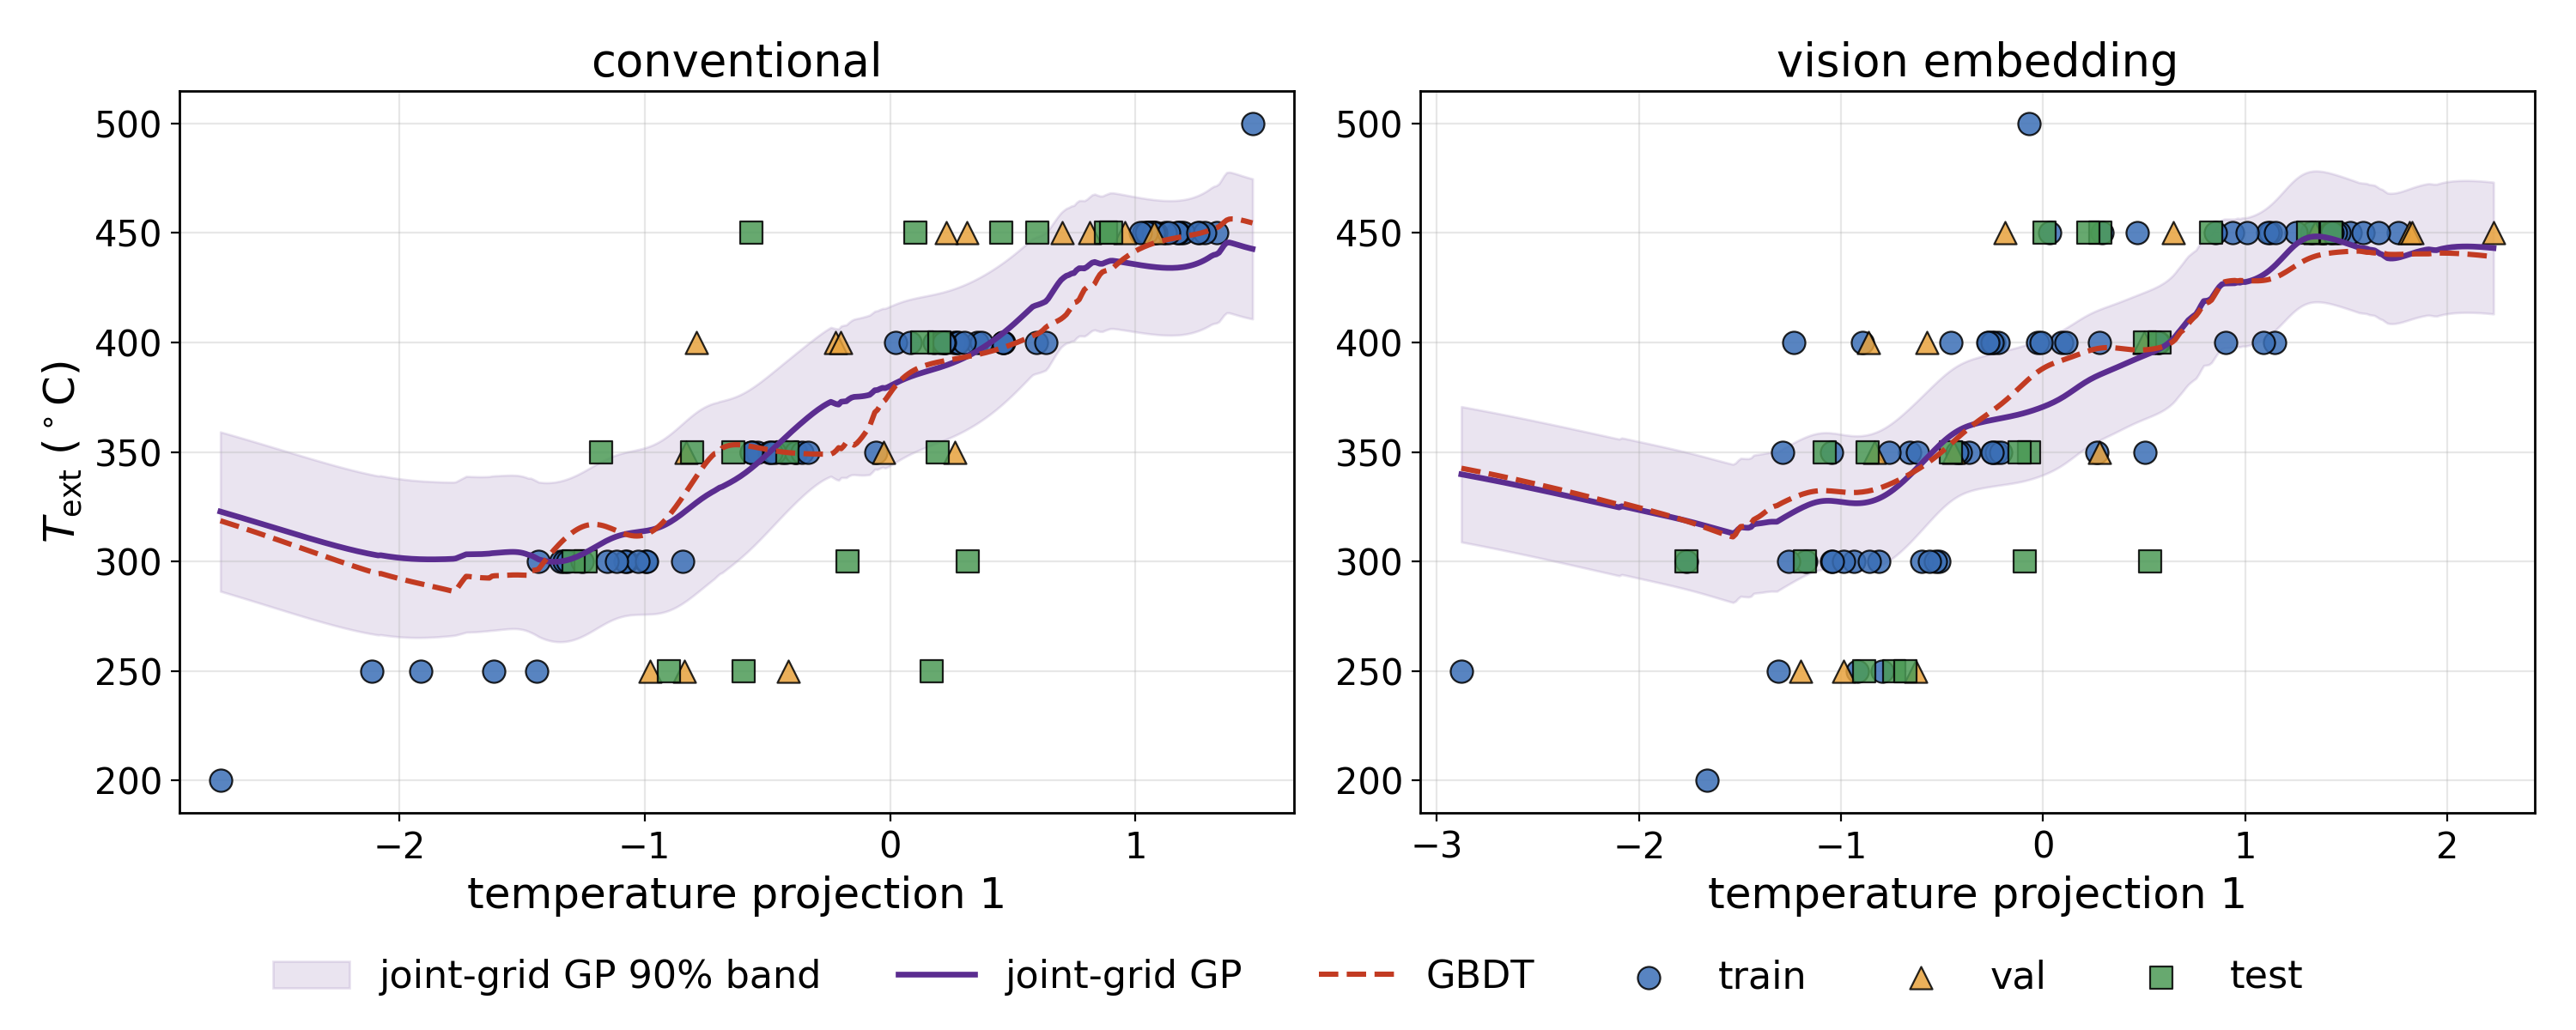
\includegraphics[width=0.99\linewidth]{figures/fig_lda_temperature.png}
  \caption{Temperature response along a supervised 1-D projection of the head
  input (selected on validation), one panel per branch. Points = conditions;
  purple curve and band = smoothed joint-grid GP mean and 90\% interval; red
  dashed = GBDT.}
  \label{fig:lda_temperature}
\end{figure}

\begin{figure}[t]
  \centering
  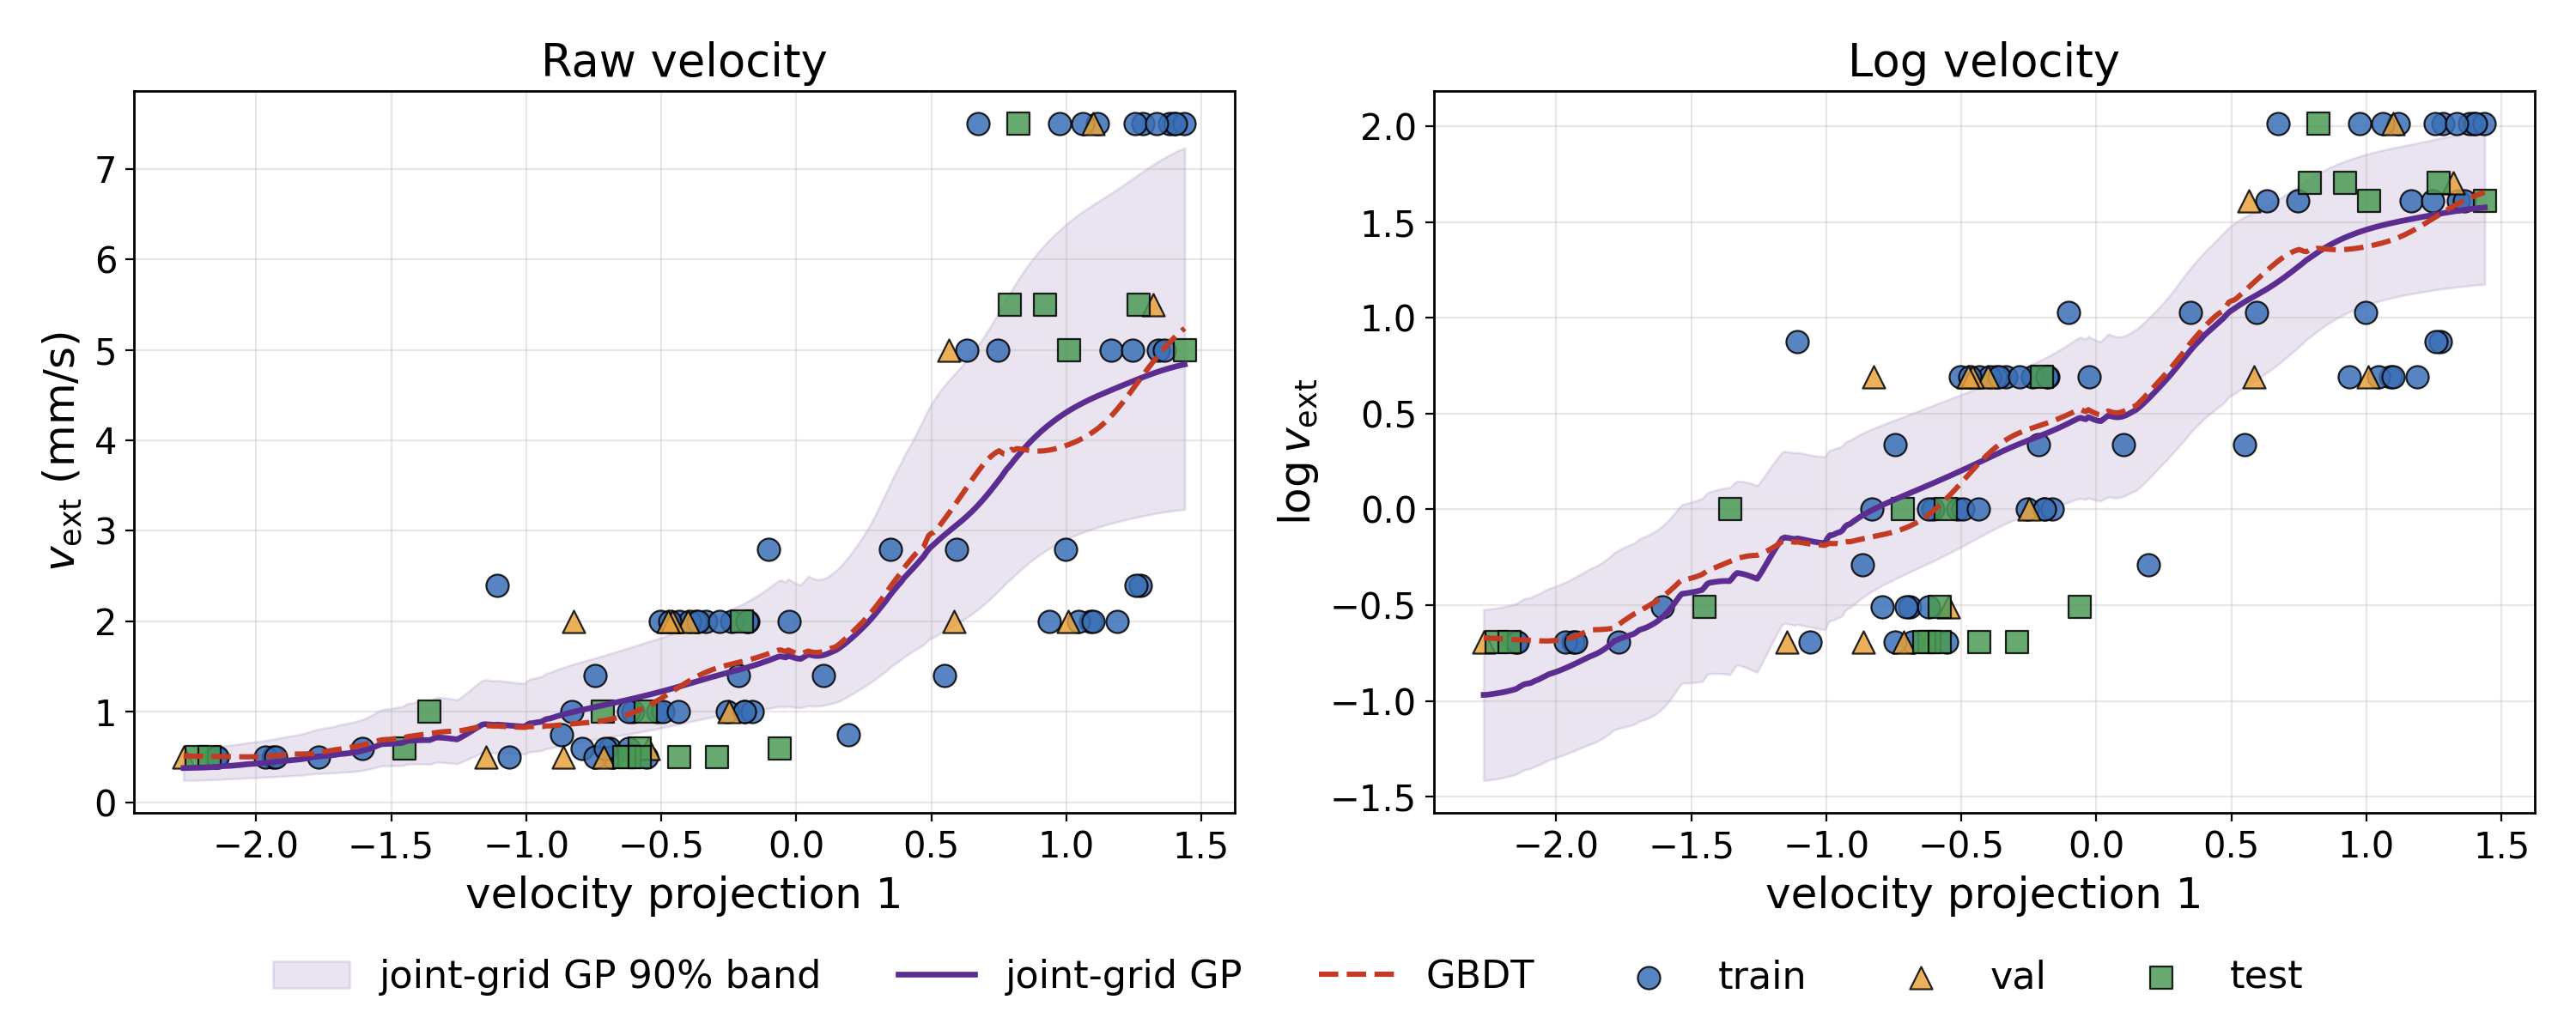
\includegraphics[width=0.99\linewidth]{figures/fig_gnn_lda_velocity.png}
  \caption{Velocity response along a supervised 1-D projection on the GNN
  branch, raw (left) and log (right). The response is a sigmoid that
  saturates at the fast end.}
  \label{fig:gnn_velocity}
\end{figure}

\begin{table}[t]
  \caption{Task B, process given known composition. 5-fold cross-validation,
  mean over held-out condition groups (std in
  Table~\ref{tab:app_process}). MAE in °C ($\Text$) or mm/s ($\vext$); log MAE
  is the velocity error in log space. Hit rate: for $\vext$ the fraction
  recovered at the exact press setting (chance 9\%); for $\Text$ the fraction
  within $\pm 25$°C. Best per representation block in bold.}
  \label{tab:process}
  \centering\small
  \begin{tabularx}{\linewidth}{@{}lllXXXX@{}}
    \toprule
    repr. & head & target & MAE & MAPE (\%) & log MAE & hit rate (\%) \\
    \midrule
    \multirow{6}{*}{conv.}
      & GBDT & $\Text$ & 41.6 & 11.9 & -- & 36 \\
      & ARD GP & $\Text$ & 52.1 & 15.2 & -- & 25 \\
      & joint-grid GP & $\Text$ & \textbf{38.1} & \textbf{10.9} & -- & \textbf{41} \\
      \cmidrule(l){2-7}
      & GBDT & $\vext$ & 1.34 & 64.5 & 0.580 & 11 \\
      & ARD GP & $\vext$ & 1.71 & 104.7 & 0.751 & 15 \\
      & joint-grid GP & $\vext$ & \textbf{0.98} & \textbf{48.7} & \textbf{0.420} & \textbf{24} \\
    \midrule
    \multirow{2}{*}{vision}
      & joint-grid GP & $\Text$ & \textbf{35.2} & \textbf{10.5} & -- & \textbf{46} \\
      & joint-grid GP & $\vext$ & \textbf{1.10} & \textbf{49.6} & \textbf{0.450} & \textbf{24} \\
    \midrule
    \multirow{2}{*}{gnn}
      & GBDT & $\Text$ & 36.5 & 10.7 & -- & 48 \\
      & joint-grid GP & $\vext$ & \textbf{1.01} & \textbf{51.4} & \textbf{0.443} & \textbf{29} \\
    \bottomrule
  \end{tabularx}
\end{table}

\paragraph{The guard metrics earn their keep.} In our head-search archive,
hurdle and metric-learning heads reached 17.0\% WAPE on a single split, close
to the reranker, while silently predicting 14\% false-positive elements and
67\% all-element WAPE. Reported with guards, they are obviously broken;
reported on WAPE alone, they would have been our headline. We keep them as a
two-sentence negative result: on a sparse lattice, any head that buys
present-element error with false presence is detectable only if all-element
error and false-positive rate travel with the headline.

\paragraph{Calibration, honestly.} The grid-GP intervals are under-dispersed
(90\% coverage $\approx$ 0.5), because the grid decode concentrates mass on
observed pairs; the plain ARD GP on gnn is the best-calibrated head (coverage
0.69 temperature, 0.71 velocity). We report both rather than smoothing the
story: the winning heads are point-accurate, and their uncertainty statements
should not be trusted beyond that.

\paragraph{Per-fold detail.}
\label{sec:perfold}
Tables~\ref{tab:app_composition} and \ref{tab:app_process}
(Appendix~\ref{app:results}) report every fold: the conventional reranker
leads on all five, and the vision/gnn rows show why the fold mean is the
honest summary (28 to 76\% WAPE on vision). The selection audit is in
\texttt{cv\_selection\_audit.csv}; all tables rebuild with
\texttt{scripts/run/run\_cv.py} and \texttt{aggregate\_cv.py}.

\section{What this means for messy real data}
\label{sec:discussion}

\paragraph{An answer to the scaling question.} At this data scale, larger
learned representations do not yield predictable improvements: the
2.5B-parameter-lineage vision embedding loses to 438 handcrafted statistics by
a factor of three on composition WAPE. The bottleneck is not model capacity but
descriptor-task compatibility: the recipe behind an optimized microstructure
lives in grain-size and shape distributions, boundary statistics, and texture
components that the handcrafted pipeline encodes explicitly and the vision
embedding retains only as needed for reconstruction. The gap should narrow as
such embeddings see larger and more diverse corpora, but on today's
campaigns the domain-designed descriptor is the right prior.

\paragraph{Practical guidance for automated characterization.} Optical
microscopy plus X-ray pole figures, the cheapest standard characterization
stack, already suffice to read the recipe back from an optimized structure:
0.65 alloy identification and a 50\%-MAPE velocity estimate from microstructure
and texture alone. In a self-driving laboratory this makes recipe recovery a
free byproduct of measurements already being collected, usable for quality
control, mislabel detection, and cross-laboratory data reconciliation
\cite{low2025selfdriving}. The guard-metric discipline
transfers directly: any characterization model deployed on sparse labels should
ship with the metrics that would expose its failure modes.

\paragraph{Limitations.} The composition lattice is a closed set of 14 alloys;
identification outside it is out of scope. The tasks are confounded by design
(families occupy process sub-grids), and condition-grouped folds remove
condition leakage but not family structure. GNN embeddings are frozen per fold,
so those rows are fixed-encoder diagnostics. Grid-GP intervals are
under-dispersed, and the velocity predictions shrink toward the centre of the
speed menu, so the extreme settings carry the largest error. And 107
conditions, however real, remain small; the dispersion across folds in
Table~\ref{tab:composition} is the honest price.

\section{Conclusion}

Which alloy composition, and what process parameters? On sparse experimental
data, the handcrafted descriptor with a lattice-aware reranked classifier
answers the first question at 13.6\% WAPE and 0.65 alloy top-1, and a
catalogue-decoding Gaussian process answers the second at 50\% velocity MAPE.
The recipe behind an optimized microstructure was never a continuous object;
the descriptors and heads that know that are the ones compatible with reading
it back.

% Bibliography. The red \needref{...} text stays inline for manual checking
% alongside the numeric \cite{...}.
\bibliographystyle{unsrtnat}
\bibliography{references}

\appendix
\section{Additional results}
\label{app:results}

This appendix collects the reproducibility details, the per-fold tables, and
the diagnostic figures that support Section~\ref{sec:results}. All quantities
are computed from the stored raw per-fold predictions under condition-grouped
5-fold cross-validation; the figures that name a single fold use
\texttt{cv\_fold0} for illustration, while the pooled figures aggregate all
107 held-out conditions.

\subsection{Reproducibility}
\label{sec:repro}

The benchmark runs as \texttt{python scripts/run/run\_cv.py} (all five folds,
three representations, both tasks) followed by \texttt{python
scripts/run/aggregate\_cv.py}, which writes the CSVs behind
Tables~\ref{tab:composition} and \ref{tab:process}. Every head stores raw
per-fold test predictions, so any metric not reported here is a recomputation,
never a re-fit. Code and split files: anonymized repository \needref{code
repository link, add at submission}.

\subsection{Per-fold tables}

\begin{table}[h]
  \caption{Task A per fold: WAPE (\%) / alloy top-1 for each of the five
  held-out condition groups.}
  \label{tab:app_composition}
  \centering\footnotesize
  \begin{tabularx}{\linewidth}{@{}llXXXXX@{}}
    \toprule
    repr. & head & fold 1 & fold 2 & fold 3 & fold 4 & fold 5 \\
    \midrule
    \multirow{3}{*}{conv.}
      & kNN & 38.1/0.35 & 20.0/0.63 & 26.6/0.50 & 28.2/0.57 & 37.2/0.43 \\
      & balanced fusion & 15.0/0.60 & 9.5/0.74 & 14.8/0.59 & 20.3/0.61 & 24.6/0.52 \\
      & OOF reranker & 9.5/0.65 & 11.4/0.68 & 13.0/0.64 & 13.6/0.70 & 20.4/0.57 \\
    \midrule
    \multirow{3}{*}{vision}
      & kNN & 39.8/0.30 & 44.7/0.42 & 75.9/0.18 & 72.9/0.26 & 52.7/0.30 \\
      & balanced fusion & 31.9/0.40 & 47.0/0.32 & 28.0/0.32 & 42.9/0.22 & 73.8/0.13 \\
      & OOF reranker & 31.9/0.40 & 31.2/0.37 & 28.0/0.32 & 42.9/0.22 & 73.8/0.13 \\
    \midrule
    \multirow{3}{*}{gnn}
      & kNN & 30.5/0.40 & 35.7/0.42 & 48.7/0.23 & 49.2/0.22 & 59.7/0.13 \\
      & balanced fusion & 31.9/0.35 & 43.9/0.32 & 46.4/0.27 & 45.4/0.22 & 54.1/0.17 \\
      & OOF reranker & 31.9/0.35 & 43.9/0.32 & 45.4/0.27 & 45.4/0.22 & 54.1/0.17 \\
    \bottomrule
  \end{tabularx}
\end{table}

\begin{table}[h]
  \caption{Task B, full 5-fold statistics (mean $\pm$ std). $\log\vext$ rows
  score the same predictions in natural-log space. MAPE itself is undefined
  there because $\log\vext$ crosses zero inside the observed range, so those
  rows instead report $100 \times$ log-space MAE, the well-defined
  first-order approximation to percent error: 42 means the typical prediction
  is off by roughly 42\%.}
  \label{tab:app_process}
  \centering\small
  \begin{tabularx}{\linewidth}{@{}lllXX@{}}
    \toprule
    repr. & head & target & MAE & MAPE (\%) \\
    \midrule
    conv. & GBDT & $\Text$ & $41.6 \pm 10.5$ & $11.9 \pm 2.3$ \\
    conv. & ARD GP & $\Text$ & $52.1 \pm 6.9$ & $15.2 \pm 2.0$ \\
    conv. & joint-grid GP & $\Text$ & $38.1 \pm 5.6$ & $10.9 \pm 1.1$ \\
    conv. & GBDT & $\vext$ & $1.34 \pm 0.33$ & $64.5 \pm 15.6$ \\
    conv. & ARD GP & $\vext$ & $1.71 \pm 0.21$ & $104.7 \pm 40.9$ \\
    conv. & joint-grid GP & $\vext$ & $0.98 \pm 0.19$ & $48.7 \pm 12.4$ \\
    conv. & GBDT & $\log\vext$ & $0.580 \pm 0.069$ & $58.0 \pm 6.9$ \\
    conv. & ARD GP & $\log\vext$ & $0.751 \pm 0.138$ & $75.1 \pm 13.8$ \\
    conv. & joint-grid GP & $\log\vext$ & $0.420 \pm 0.083$ & $42.0 \pm 8.3$ \\
    \midrule
    vision & GBDT & $\Text$ & $39.2 \pm 10.1$ & $11.4 \pm 1.9$ \\
    vision & ARD GP & $\Text$ & $72.1 \pm 18.0$ & $19.9 \pm 3.4$ \\
    vision & joint-grid GP & $\Text$ & $35.2 \pm 7.3$ & $10.5 \pm 1.4$ \\
    vision & GBDT & $\vext$ & $1.22 \pm 0.32$ & $55.9 \pm 10.7$ \\
    vision & ARD GP & $\vext$ & $1.76 \pm 0.53$ & $120.5 \pm 57.2$ \\
    vision & joint-grid GP & $\vext$ & $1.10 \pm 0.24$ & $49.6 \pm 14.5$ \\
    vision & GBDT & $\log\vext$ & $0.491 \pm 0.051$ & $49.1 \pm 5.1$ \\
    vision & ARD GP & $\log\vext$ & $0.742 \pm 0.279$ & $74.2 \pm 27.9$ \\
    vision & joint-grid GP & $\log\vext$ & $0.450 \pm 0.109$ & $45.0 \pm 10.9$ \\
    \midrule
    gnn & GBDT & $\Text$ & $36.5 \pm 10.1$ & $10.7 \pm 2.2$ \\
    gnn & ARD GP & $\Text$ & $49.5 \pm 8.9$ & $14.7 \pm 3.1$ \\
    gnn & joint-grid GP & $\Text$ & $36.6 \pm 7.8$ & $10.8 \pm 1.9$ \\
    gnn & GBDT & $\vext$ & $1.11 \pm 0.33$ & $56.0 \pm 16.8$ \\
    gnn & ARD GP & $\vext$ & $1.44 \pm 0.16$ & $94.5 \pm 38.8$ \\
    gnn & joint-grid GP & $\vext$ & $1.01 \pm 0.26$ & $51.4 \pm 13.9$ \\
    gnn & GBDT & $\log\vext$ & $0.475 \pm 0.085$ & $47.5 \pm 8.5$ \\
    gnn & ARD GP & $\log\vext$ & $0.626 \pm 0.112$ & $62.6 \pm 11.2$ \\
    gnn & joint-grid GP & $\log\vext$ & $0.443 \pm 0.059$ & $44.3 \pm 5.9$ \\
    \bottomrule
  \end{tabularx}
\end{table}

\subsection{Composition diagnostics}

Figure~\ref{fig:app_taxonomy} breaks the top-1 alloy call down by alloy, and
Figure~\ref{fig:app_elements} the element-level error behind the WAPE in
Table~\ref{tab:composition}. Together they show the branches differ in
concentration resolution, not in recognising the alloy system.

\begin{figure}[h]
  \centering
  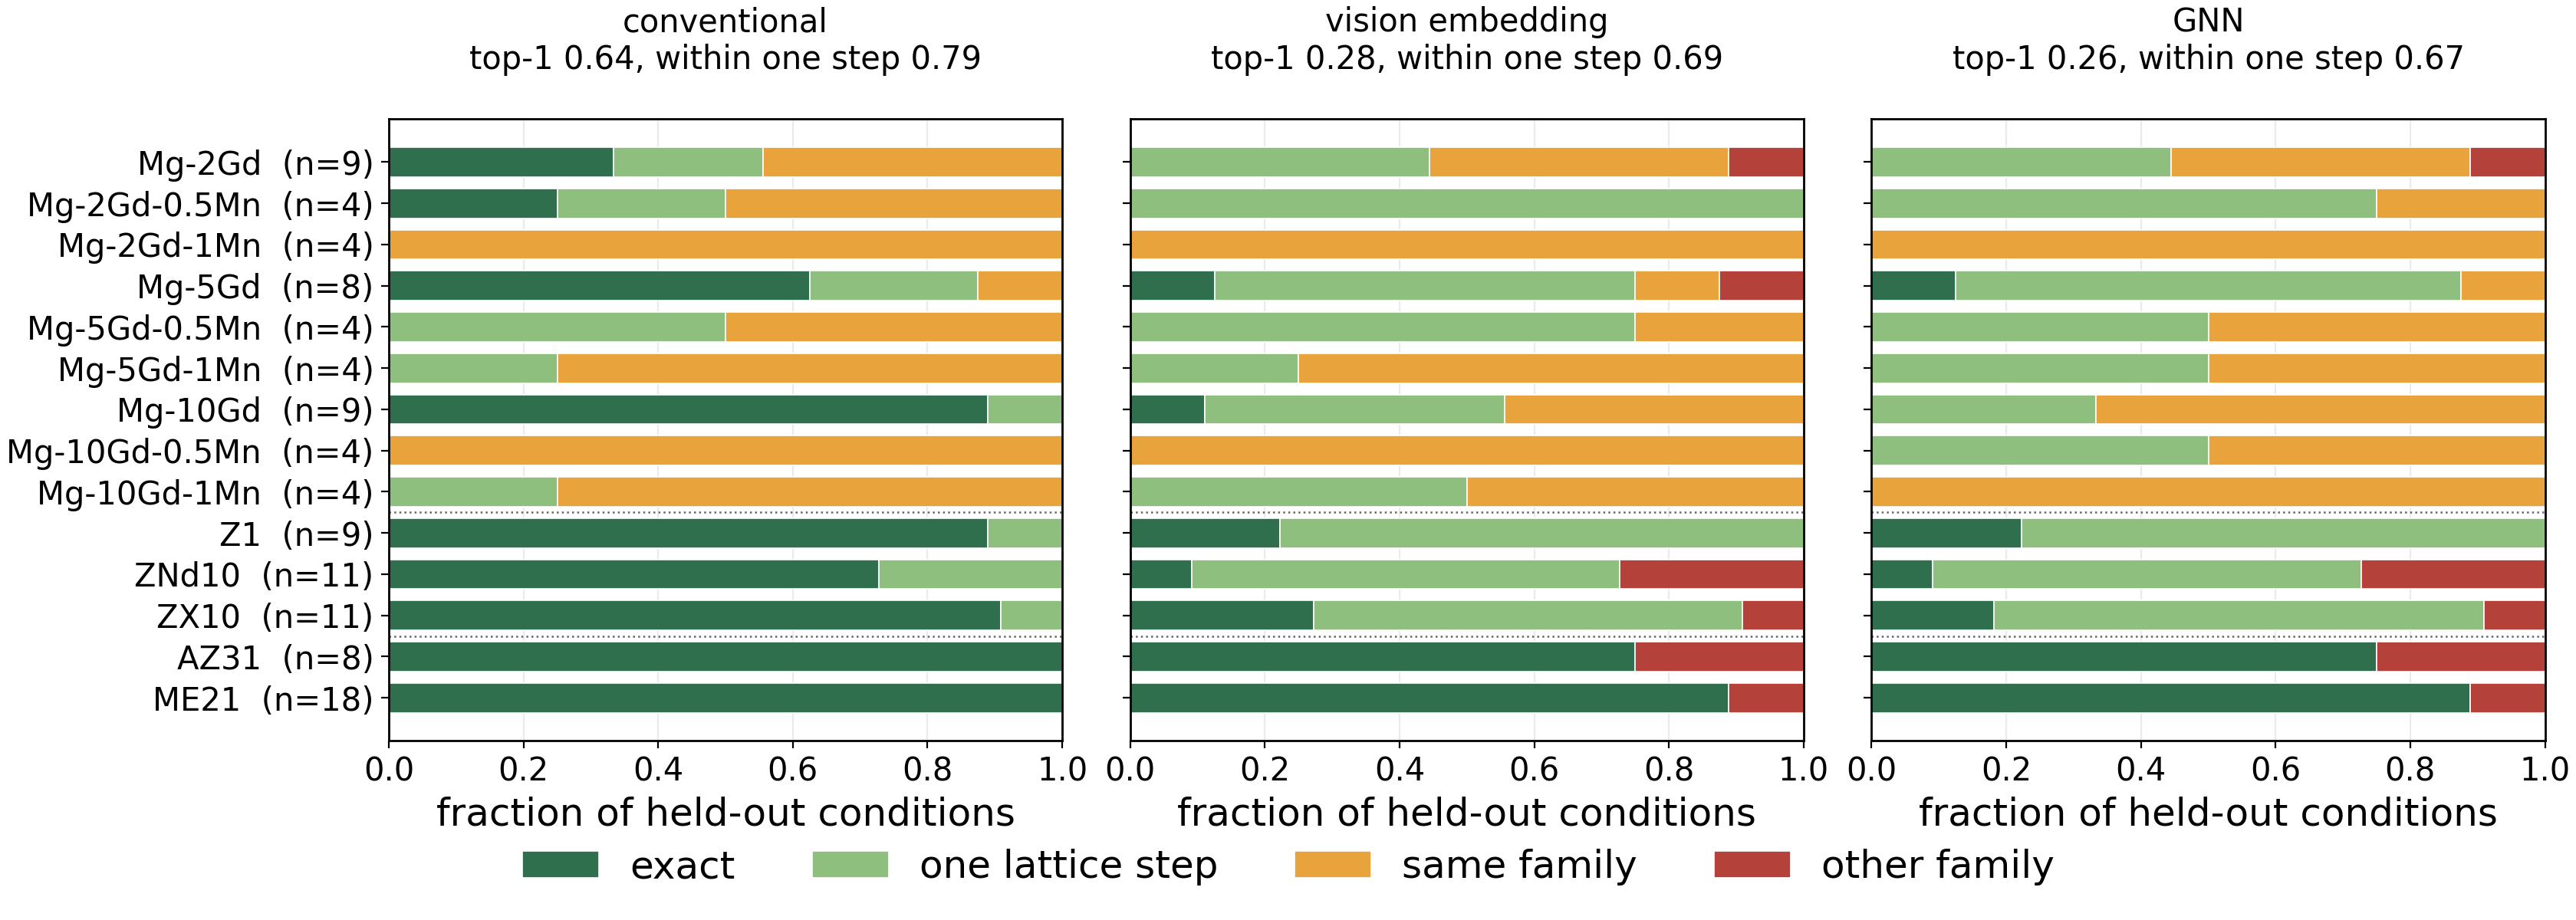
\includegraphics[width=0.99\linewidth]{figures/fig_composition_taxonomy.png}
  \caption{Where the top-1 alloy call lands, per alloy, pooled over all 107
  held-out conditions. One lattice step is one Gd or one Mn step inside the
  Mg-Gd(-Mn) grid, or a swap within the Z1 / ZNd10 / ZX10 trio. Conventional
  is exact on AZ31 and ME21 and nearly all of its misses are one lattice step
  (within one step 0.79 against a top-1 of 0.64); the embeddings stay near
  0.68 within one step, so the gap is in resolving concentration, not
  chemistry. Rows have small and unequal n (4 to 18), so a single
  misclassified condition moves a small-n alloy's bar by 25\%.}
  \label{fig:app_taxonomy}
\end{figure}

\begin{figure}[h]
  \centering
  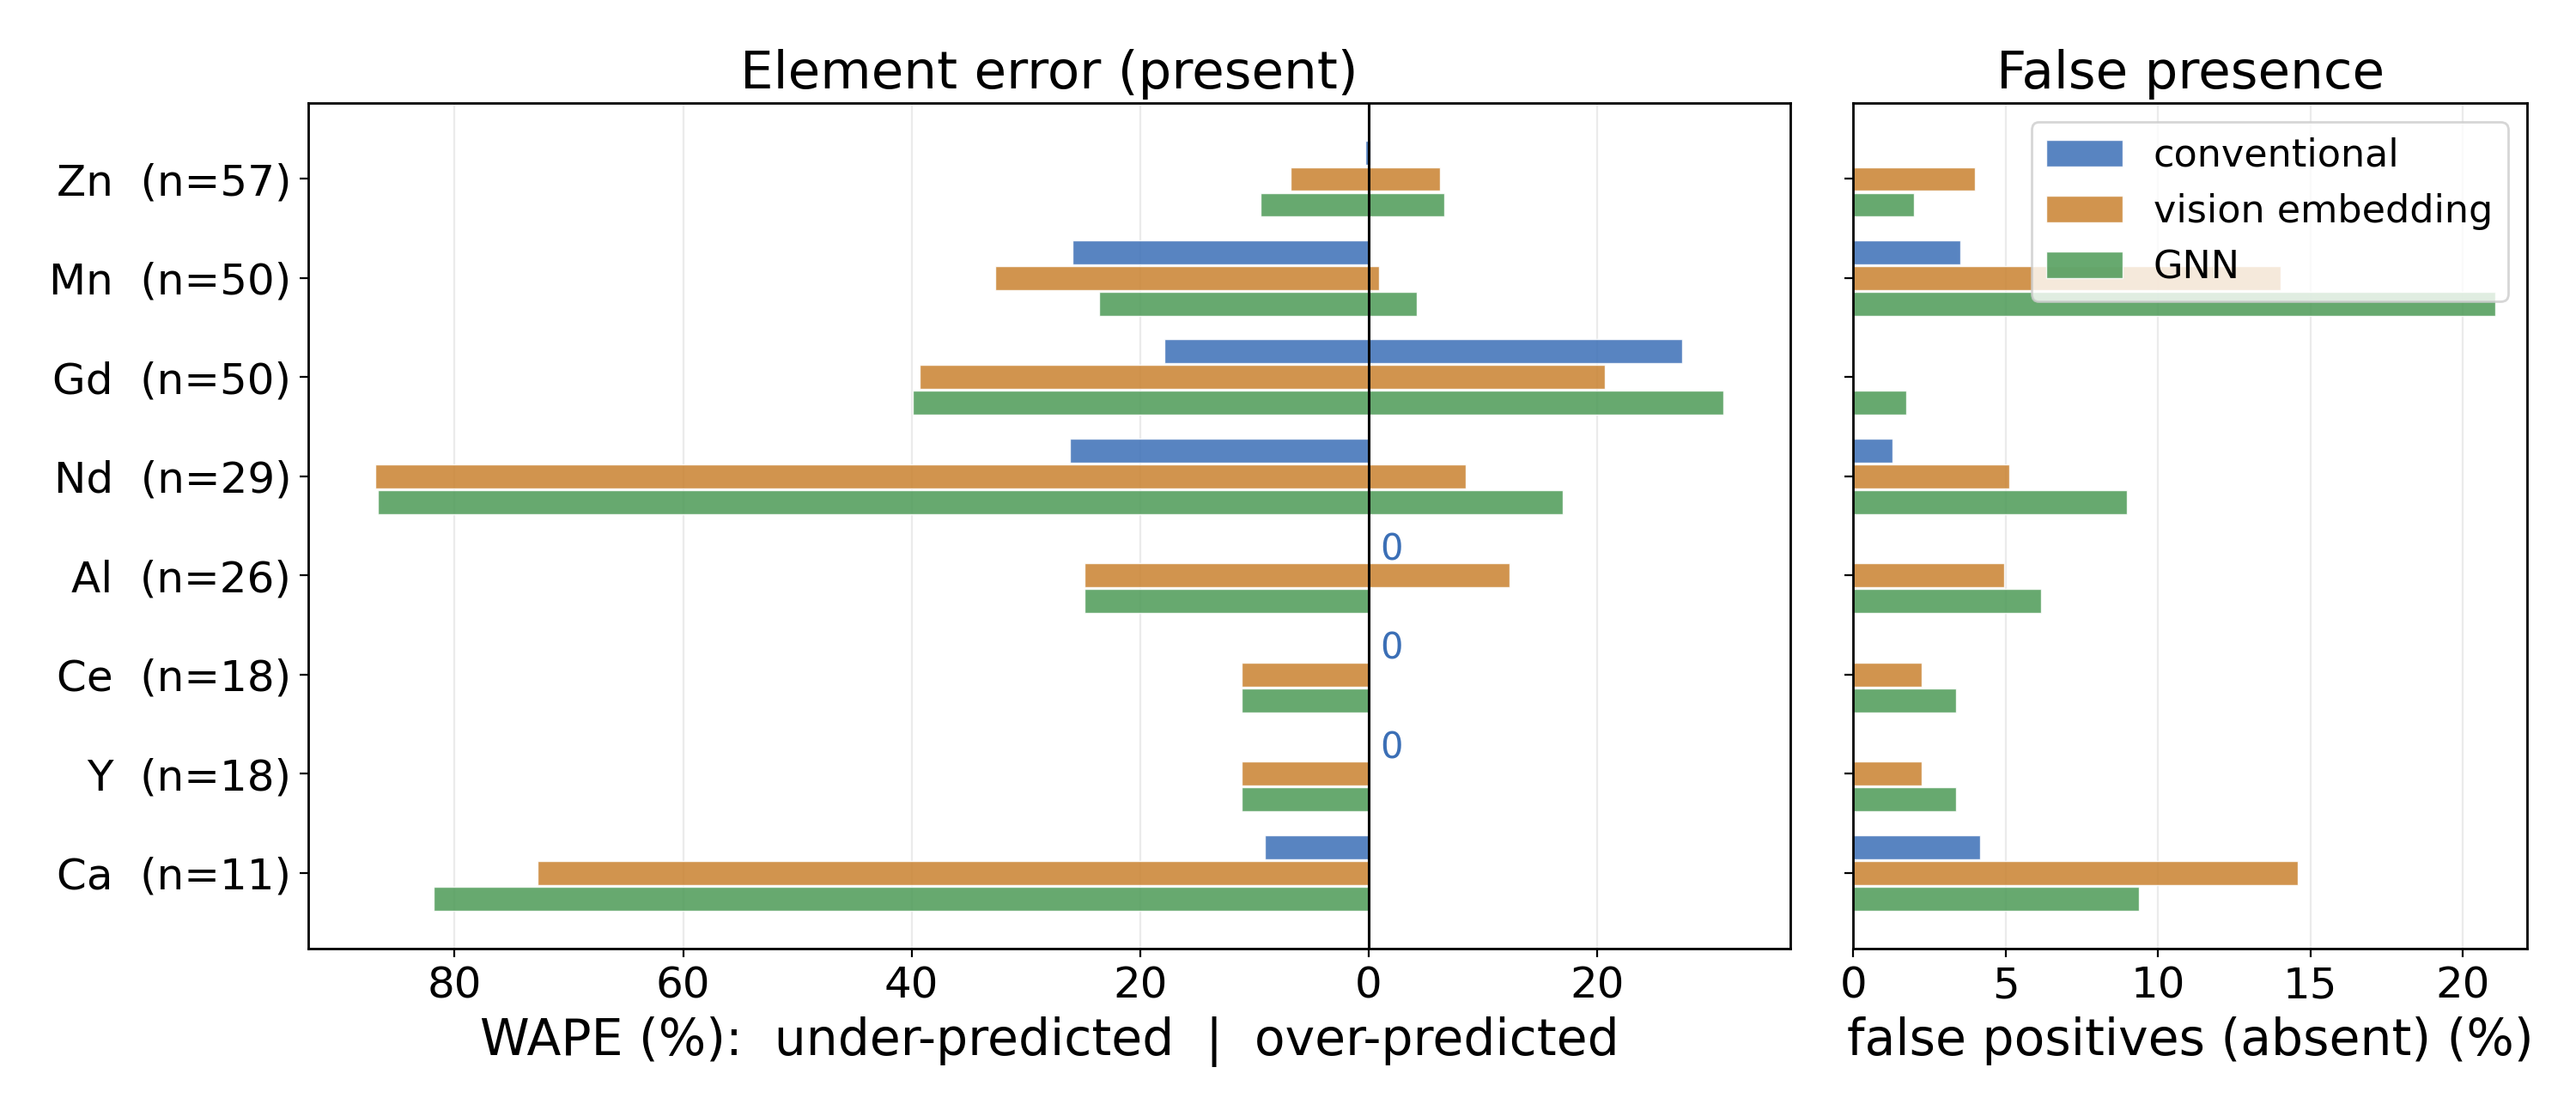
\includegraphics[width=0.99\linewidth]{figures/fig_composition_elements.png}
  \caption{Per-element error. Left: per-element WAPE where the element is
  present, split at zero into the under-predicted and over-predicted share; a
  ``0'' marks a branch exactly right on every condition containing that
  element. Right: the presence false-positive rate. Conventional is exact on
  Zn, Al, Ce and Y, so its error sits in Gd, Mn, Nd and Ca; the embeddings
  under-predict the rare elements (Nd and Ca) yet over-predict Mn and Ca where
  they are absent. Because the head decodes to a lattice alloy, per-element
  error takes only a few exact values, so bars are used rather than a density.}
  \label{fig:app_elements}
\end{figure}

\subsection{Process diagnostics}

Figures~\ref{fig:app_conv_velocity} and \ref{fig:app_conv_vel_parity} repeat
the GNN velocity analysis of Figures~\ref{fig:gnn_velocity} and
\ref{fig:vel_parity} on the conventional branch, and
Figure~\ref{fig:app_gnn_projection} shows the underlying 2-D velocity
embedding.

\begin{figure}[h]
  \centering
  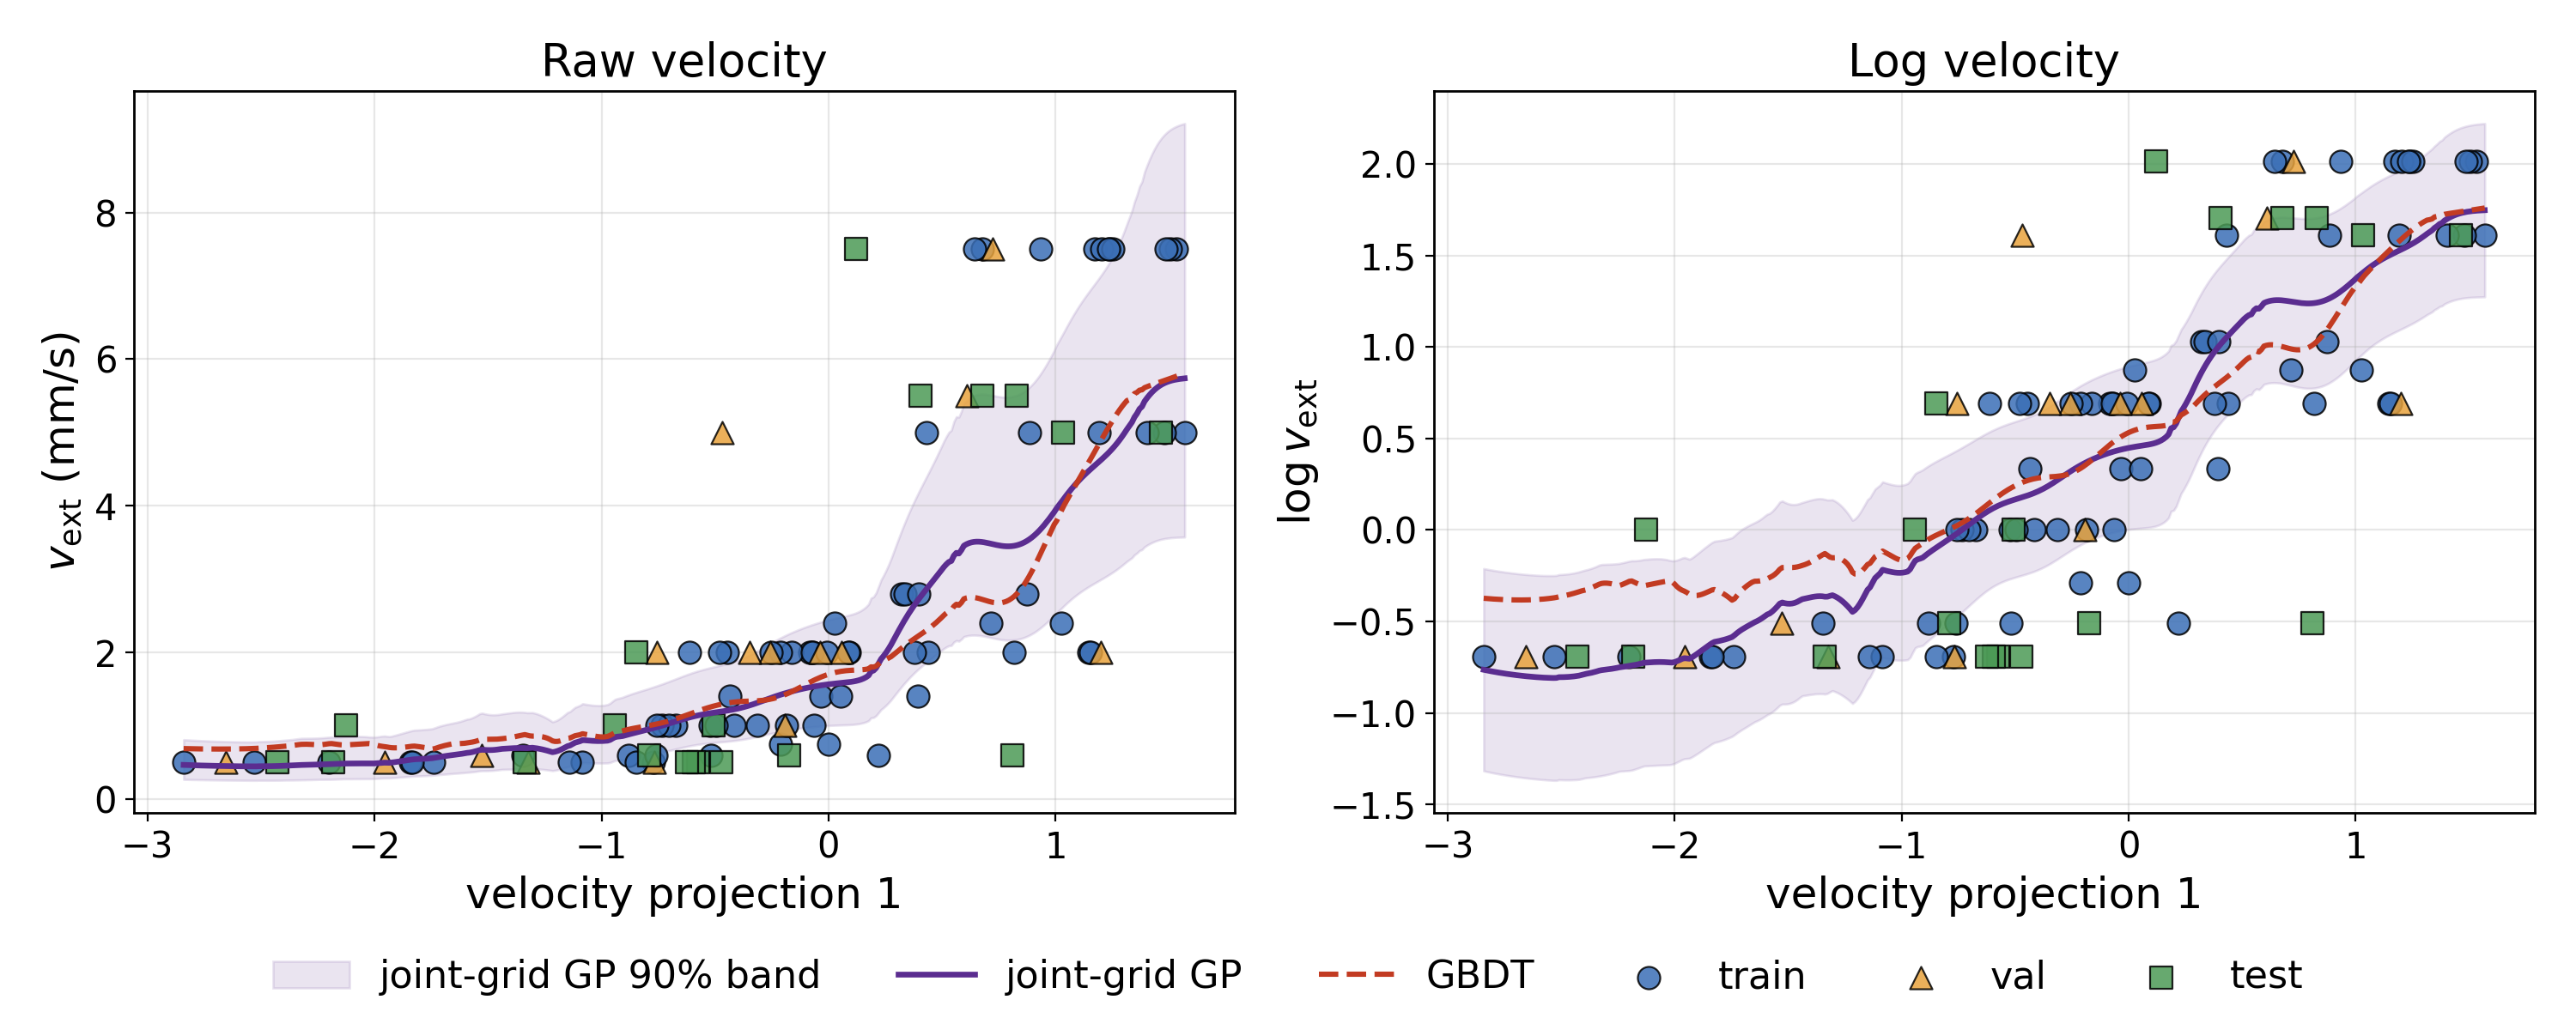
\includegraphics[width=0.99\linewidth]{figures/fig_conventional_lda_velocity.png}
  \caption{Velocity response along a supervised 1-D projection on the
  conventional branch, raw (left) and log (right). The conventional projection
  is dominated by a single extreme low-velocity cluster (projection
  $\approx -3$), so it is less well behaved than the GNN axis in
  Figure~\ref{fig:gnn_velocity}; the sigmoid shape and the saturation at the
  fast end are otherwise the same.}
  \label{fig:app_conv_velocity}
\end{figure}

\begin{figure}[h]
  \centering
  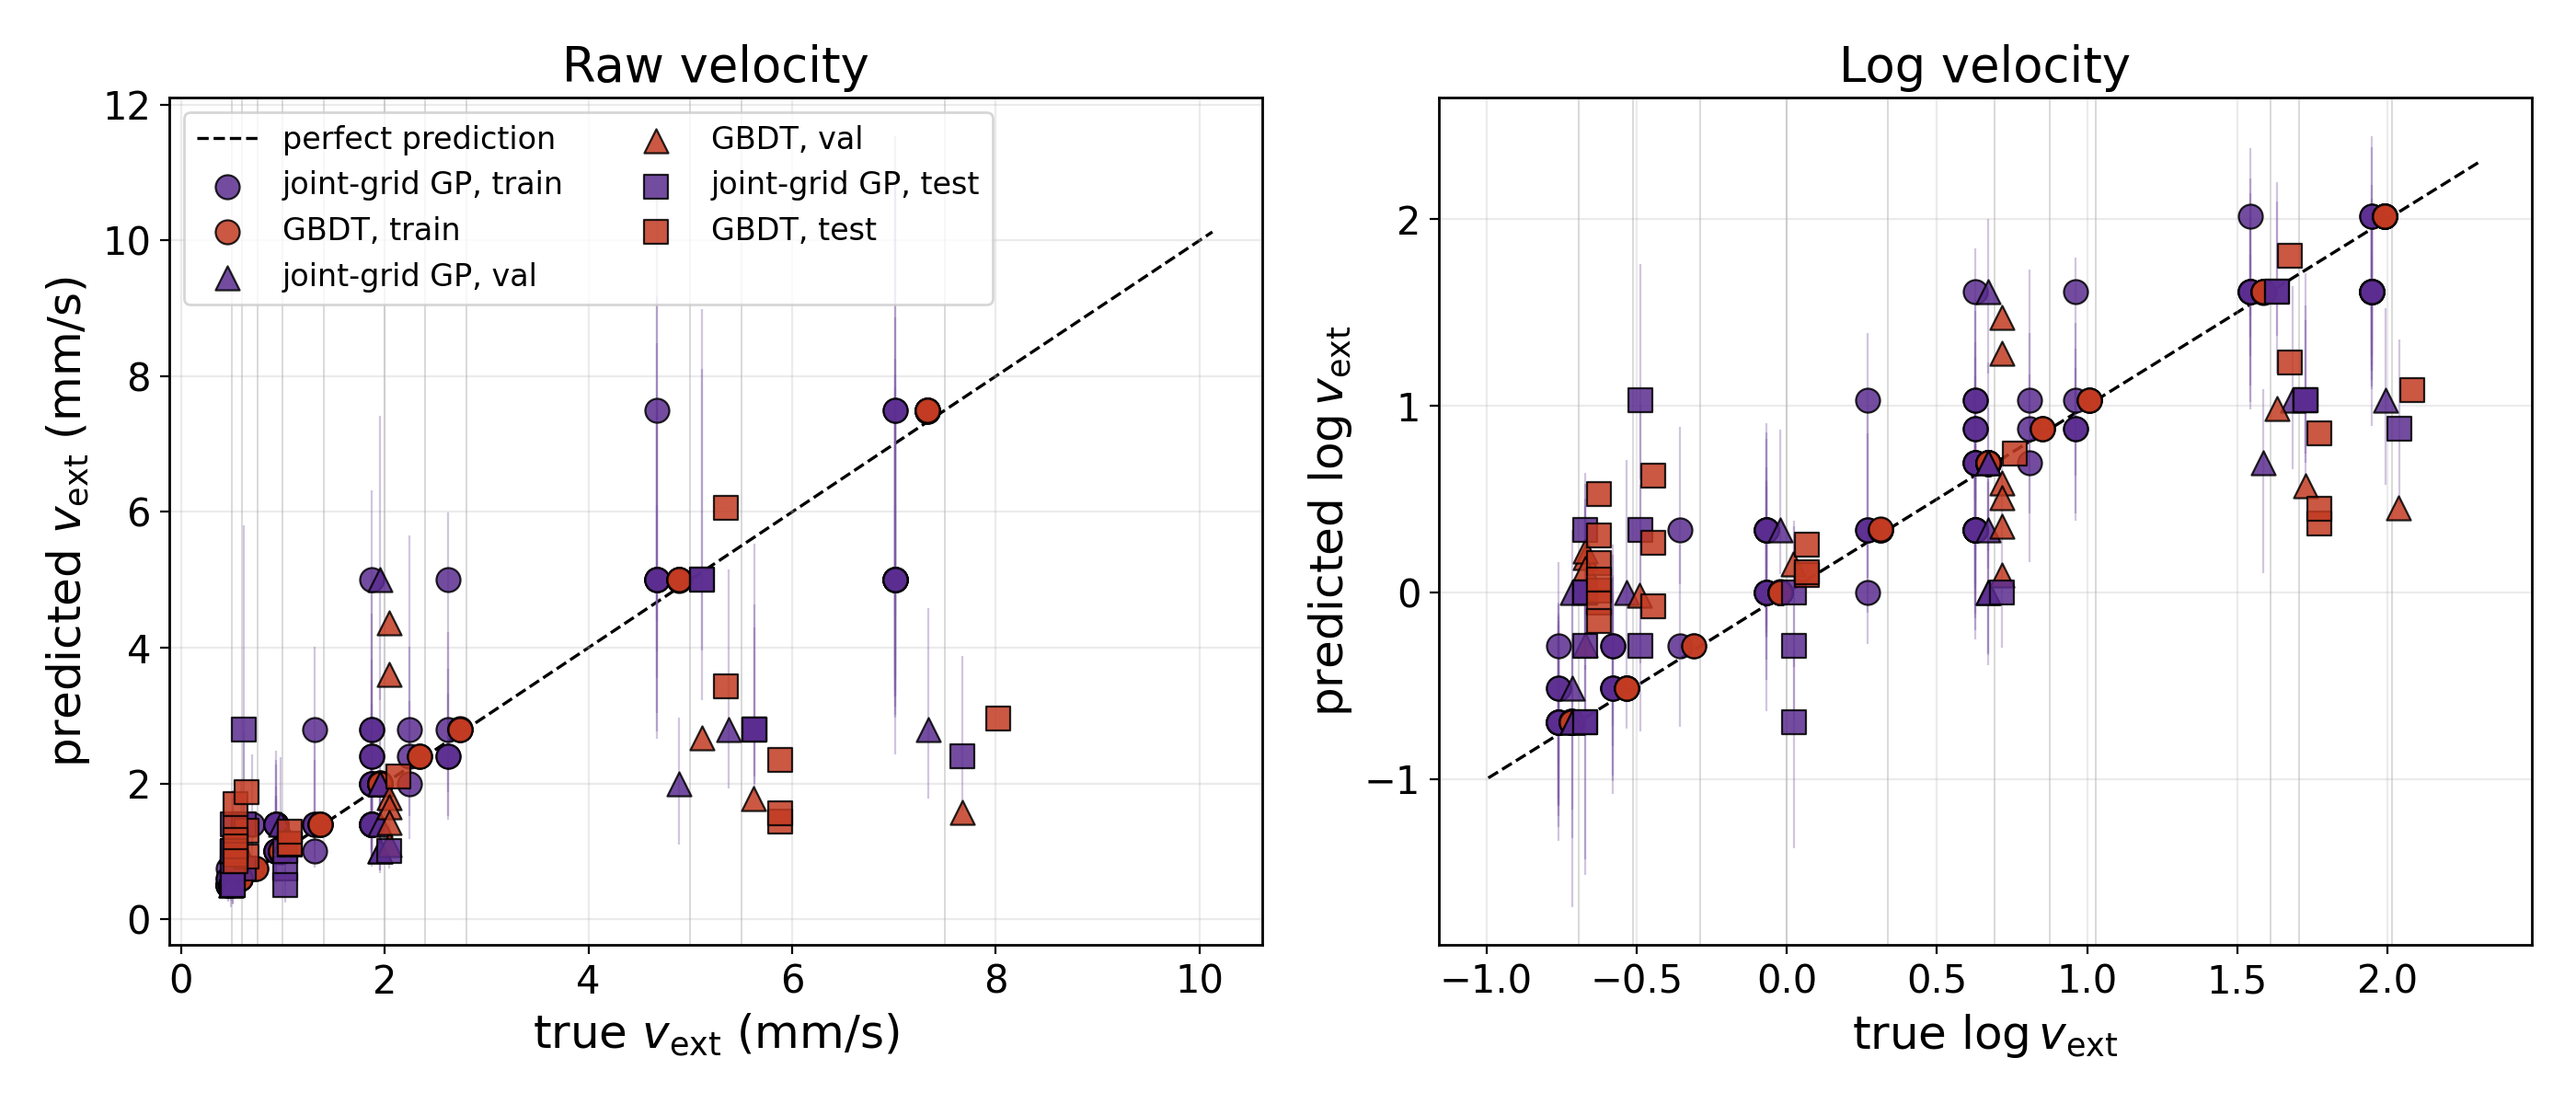
\includegraphics[width=0.99\linewidth]{figures/fig_conventional_velocity_parity.png}
  \caption{Velocity parity on the conventional branch (\texttt{cv\_fold0}),
  raw (left) and log (right), matching Figure~\ref{fig:vel_parity}. The same
  tight-at-low-speed, undershoot-at-high-speed pattern holds.}
  \label{fig:app_conv_vel_parity}
\end{figure}

\begin{figure}[h]
  \centering
  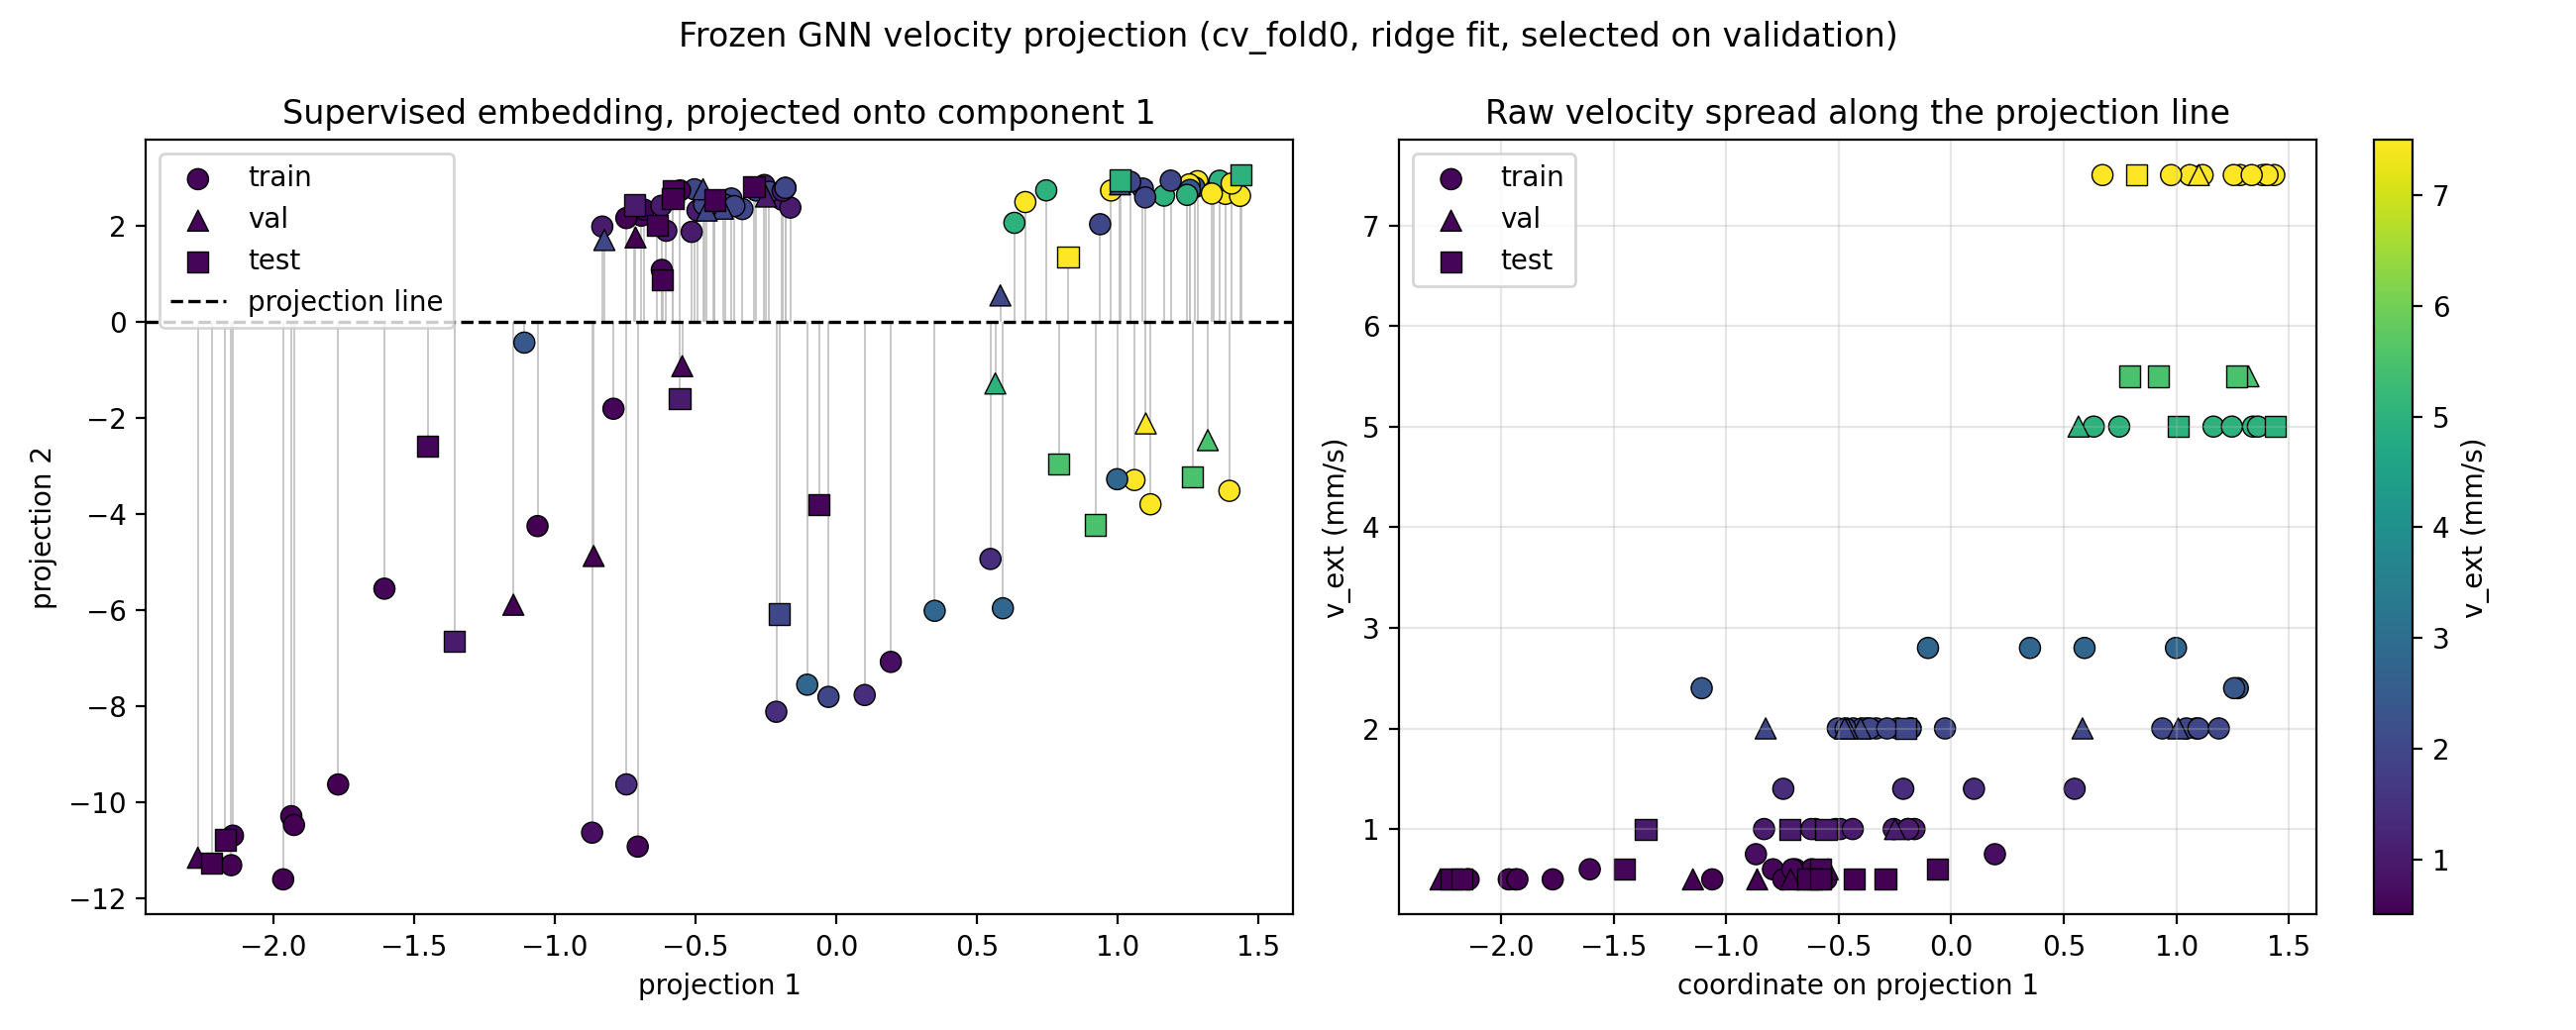
\includegraphics[width=0.99\linewidth]{figures/fig_gnn_lda_projection.png}
  \caption{The frozen GNN velocity projection (\texttt{cv\_fold0}). Left: the
  2-D supervised embedding, points coloured by true $\vext$, with each point
  joined to the projection line. Right: the raw velocity spread along
  component 1. The projection separates the slow conditions but compresses the
  fast ones, which is why the 1-D response in Figure~\ref{fig:gnn_velocity}
  saturates.}
  \label{fig:app_gnn_projection}
\end{figure}

\end{document}
